\documentclass[a4paper,USenglish]{lipics-v2016-utf8x}

\usepackage{amsthm,amstext,amssymb,amsmath}
\usepackage{datetime}
\usepackage{fdsymbol} %% must be loaded before bbold because it interferes with numbers
\usepackage{bbold}
\usepackage{url}
\usepackage{xcolor}
\usepackage{multicol}
\usepackage{proof}
\usepackage{stmaryrd}
\usepackage{bussproofs}
\usepackage{tikz}
\usepackage{tikz-cd}
\usetikzlibrary{quotes}
\usepackage[section]{placeins}
\usepackage{braket}

\newcommand{\textpi}{$\pi$}
\newcommand{\ft}{\mathbb{T}}
\newcommand{\hash}{\#}
\newcommand{\pifrac}{\ensuremath{\Pi^/}}
\newcommand{\iso}{\leftrightarrow}
\newcommand{\isotwo}{\Leftrightarrow}
\newcommand{\alt}{~|~}
\newcommand{\ag}[2]{#1 \sslash #2}
\newcommand{\agp}[3]{#1 \sslash_{#3} #2}
\newcommand{\order}[1]{\hash #1}
\newcommand{\iorder}[1]{1/\hash #1}
\newcommand{\oneg}[1]{\mathbb{1}_{#1}}
\newcommand{\divgl}[2]{\hash{#1} \div_{l} \hash{#2}}
\newcommand{\divgr}[2]{\hash{#1} \div_{r} \hash{#2}}
\newcommand{\ord}[1]{\ensuremath{\mathsf{order}(#1)}}
\newcommand{\inl}[1]{\textsf{inl}(#1)}
\newcommand{\inr}[1]{\textsf{inr}(#1)}
\newcommand{\zt}{\mathbb{0}}
\newcommand{\ot}{\mathbb{1}}
\newcommand{\G}{\mathcal{G}}
\newcommand{\Z}{\mathbb{Z}}
\newcommand{\Zn}{\mathbb{Z}_n}
\newcommand{\Zvn}{\mathbb{Z}^v_n}
\newcommand{\N}{\mathbb{N}}
\newcommand{\cycle}{\textsf{cycle}}
\newcommand{\twod}{\mathbb{T}}
\newcommand{\fract}[2]{#1/#2}
\newcommand{\fv}[2]{\fcolorbox{black}{white}{\strut $#1$}\fcolorbox{black}{gray!20}{$\strut #2$}}
\newcommand{\pt}[2]{\bullet[#1,#2]}
\newcommand{\sing}[1]{\textsc{Sing}(#1)}
\newcommand{\singi}[2]{\textsc{SingI}_{{#1}}(#2)}
\newcommand{\iter}[1]{\textsc{Iter}(#1)}
\newcommand{\pair}[2]{\langle #1,#2 \rangle}
\newcommand{\triple}[3]{\langle #1,#2,#3 \rangle}
\newcommand{\distiterplus}[3]{\mathsf{dist}~#1~#2~#3}
\newcommand{\looping}[1]{\mathcal{L}{#1}}
\newcommand{\delooping}[1]{\mathcal{B}{#1}}

\newcommand{\permone}{\mathit{perm}_{...}}
\newcommand{\permtwo}{\mathit{perm}_{\times\!\times.}}
\newcommand{\permthree}{\mathit{perm}_{.\times\!\times}}
\newcommand{\permfour}{\mathit{perm}_{\rightarrow}}
\newcommand{\permfive}{\mathit{perm}_{\leftarrow}}
\newcommand{\permsix}{\mathit{perm}_{\times.\times}}

\newcommand{\Rule}[4]{
\makebox{{\rm #1}
$\displaystyle
\frac{\begin{array}{l}#2\\\end{array}}
{\begin{array}{l}#3\\\end{array}}$
 #4}}
\newcommand{\proves}{\vdash}
\newcommand{\jdg}[3]{{#1} #3}
\newcommand{\evalone}[2]{#1~\triangleright~#2}
\newcommand{\evaloneb}[2]{#1~\triangleleft~#2}
\newcommand{\unitv}{()}
\newcommand{\synchl}{\mathsf{{synchl}}}
\newcommand{\synchr}{\mathsf{{synchr}}}
\newcommand{\packl}{\mathsf{{packl}}}
\newcommand{\packr}{\mathsf{{packr}}}
\newcommand{\unitepl}{\mathsf{{unite_+l}}}
\newcommand{\unitipl}{\mathsf{{uniti_+l}}}
\newcommand{\unitepr}{\mathsf{{unite_+r}}}
\newcommand{\unitipr}{\mathsf{{uniti_+r}}}
\newcommand{\swapp}{\mathsf{{swap_+}}}
\newcommand{\assoclp}{\mathsf{{assocl_+}}}
\newcommand{\assocrp}{\mathsf{{assocr_+}}}
\newcommand{\unitetl}{\mathsf{{unite_{\star}l}}}
\newcommand{\unititl}{\mathsf{{uniti_{\star}l}}}
\newcommand{\unitetr}{\mathsf{{unite_{\star}r}}}
\newcommand{\unititr}{\mathsf{{uniti_{\star}r}}}
\newcommand{\swapt}{\mathsf{{swap_{\star}}}}
\newcommand{\assoclt}{\mathsf{{assocl_{\star}}}}
\newcommand{\assocrt}{\mathsf{{assocr_{\star}}}}
\newcommand{\absorbr}{\mathsf{{absorbr}}}
\newcommand{\absorbl}{\mathsf{{absorbl}}}
\newcommand{\factorzr}{\mathsf{{factorzr}}}
\newcommand{\factorzl}{\mathsf{{factorzl}}}
\newcommand{\dist}{\mathsf{{dist}}}
\newcommand{\factor}{\mathsf{{factor}}}
\newcommand{\distl}{\mathsf{{distl}}}
\newcommand{\factorl}{\mathsf{{factorl}}}
\newcommand{\idiso}{\mathsf{{id}}}

\newcommand{\assocdl}{\mathsf{{assoc_{\odot}l}}}
\newcommand{\assocdr}{\mathsf{{assoc_{\odot}r}}}
\newcommand{\idldl}{\mathsf{{idl_{\odot}l}}}
\newcommand{\idldr}{\mathsf{{idl_{\odot}r}}}
\newcommand{\idrdl}{\mathsf{{idr_{\odot}l}}}
\newcommand{\idrdr}{\mathsf{{idr_{\odot}r}}}
\newcommand{\rinvdl}{\mathsf{{rinv_{\odot}l}}}
\newcommand{\rinvdr}{\mathsf{{rinv_{\odot}r}}}
\newcommand{\linvdl}{\mathsf{{linv_{\odot}l}}}
\newcommand{\linvdr}{\mathsf{{linv_{\odot}r}}}
\newcommand{\idisotwo}{\mathsf{{id}}}
\newcommand{\transtwo}{\bullet}
\newcommand{\respstwo}{\mathsf{{\boxdot}}}
\newcommand{\respptwo}{\mathsf{{resp_{\oplus\Leftrightarrow}}}}
\newcommand{\respttwo}{\mathsf{{resp_{\otimes\Leftrightarrow}}}}
\newcommand{\sumid}{\mathsf{sumid}}
\newcommand{\splitid}{\mathsf{splitid}}
\newcommand{\homps}{\mathsf{hom_{\oplus\odot}}}
\newcommand{\homsp}{\mathsf{hom_{\odot\oplus}}}

\newcommand{\sem}[1]{\llbracket #1 \rrbracket}

\newtheorem{proposition}{Proposition}

\makeatletter
\tikzset{my loop/.style =  {to path={
  \pgfextra{\let\tikztotarget=\tikztostart}
  [looseness=8,min distance=5mm, in=240,out=300]
  \tikz@to@curve@path}
  }}
\makeatletter

%%%%%%%%%%%%%%%%%%%%%%%%%%%%%%%%%%%%%%%%%%%%%%%%%%%%%%%%%%%%%%%%%%%%%%%%%%%%%%
\begin{document}

\title{Fractional Types}
\titlerunning{Fractional Types}
\author[1]{Jacques Carette}
\author[2]{Chao-Hong Chen}
\author[3]{Vikraman Choudhury}
\author[4]{Amr Sabry}
\affil[1]{Computing and Software Department, McMaster University,
  Hamilton, Ontario, Canada \\ \texttt{carette@mcmaster.ca}}
\affil[2]{Computer Science Department, Indiana University,
  Bloomington, Indiana, USA \\ \texttt{chen464@indiana.edu}}
\affil[3]{Computer Science Department, Indiana University,
  Bloomington, Indiana, USA \\ \texttt{vikraman@indiana.edu}}
\affil[4]{Computer Science Department, Indiana University,
  Bloomington, Indiana, USA \\ \texttt{sabry@indiana.edu}}

\authorrunning{J. Carette, C.-H. Chen, V. Choudhury and A. Sabry}

\Copyright{Jacques Carette, Chao-Hong Chen, Vikraman Choudhury and Amr Sabry}

\maketitle

\begin{abstract}
We exhibit types whose natural cardinality is fractional.  More
precisely, we show that the groupoid cardinality (as defined by
Baez-Dolan) of the denotation of the type of a singleton reversible
program $p$ with exactly $k$ distinct proofs of reversibility has
cardinality $1/k$.  We further show that this type is naturally a
multiplicative inverse to the type of all iterates $p ^ i$ of that
reversible program.

We situate this work as an extension of a larger reversible
programming language ($\Pi$), and show that this extension is also
reversible.  Interestingly, this extension supports first-class
functions as well as some natural analogues of operations coming from
compact closed categories.  We emphasize that the key ingredients are
reversibility and proof relevance: cardinality $1/k$ arises from
having exactly $k$ proofs of reversibility.
\end{abstract}

%%%%%%%%%%%%%%%%%%%%%%%%%%%%%%%%%%%%%%%%%%%%%%%%%%%%%%%%%%%%%%%%%%%%%%%%%%%%%%
\section{Introduction}

In modern treatments of type theory, types have the
structure of \emph{weak $\omega$-groupoids}. As a first approximation,
we can think of such structures as sets with points (objects) and
paths (equivalences) between the points and higher paths between these
paths and so on. Here are two simple but non-trivial examples:

\begin{center}
\begin{tabular}{c@{\qquad\qquad}c}
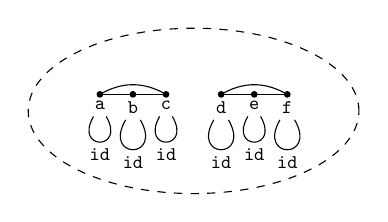
\begin{tikzpicture}[scale=0.7,every node/.style={scale=0.7}]
  \draw[dashed] (0,0) ellipse (3cm and 1.5cm);
  \node[below] (A) at (-1.7,0.3) {\texttt{a}};
  \node[below] (B) at (-1.1,0.3) {\texttt{b}};
  \node[below] (C) at (-0.5,0.3) {\texttt{c}};
  \node[below] (D) at (0.5,0.3) {\texttt{d}};
  \node[below] (E) at (1.1,0.3) {\texttt{e}};
  \node[below] (F) at (1.7,0.3) {\texttt{f}};
  \draw[fill] (-1.7,0.3) circle [radius=0.05];
  \draw[fill] (-1.1,0.3) circle [radius=0.05];
  \draw[fill] (-0.5,0.3) circle [radius=0.05];
  \draw[fill] (0.5,0.3) circle [radius=0.05];
  \draw[fill] (1.1,0.3) circle [radius=0.05];
  \draw[fill] (1.7,0.3) circle [radius=0.05];
  \draw (-1.7,0.3) -- (-1.1,0.3);
  \draw (-1.1,0.3) -- (-0.5,0.3);
  \draw (-1.7,0.3) to[bend left] (-0.5,0.3) ;
  \draw (0.5,0.3) -- (1.1,0.3);
  \draw (1.1,0.3) -- (1.7,0.3);
  \draw (0.5,0.3) to[bend left] (1.7,0.3) ;
  \path (A) edge [my loop] node[below] {\texttt{id}} (B);
  \path (B) edge [my loop] node[below] {\texttt{id}} (B);
  \path (C) edge [my loop] node[below] {\texttt{id}} (B);
  \path (D) edge [my loop] node[below] {\texttt{id}} (B);
  \path (E) edge [my loop] node[below] {\texttt{id}} (B);
  \path (F) edge [my loop] node[below] {\texttt{id}} (B);
\end{tikzpicture}
&
\begin{tikzpicture}[scale=0.6,every node/.style={scale=0.6}]
  \draw[dashed] (0,0) ellipse (2cm and 2.6cm);
  \node[below] (B) at (0,-1.1) {\texttt{*}};
  \path (B) edge [my loop] node[below] {\texttt{id}} (B);
  \path (B) edge [loop above, looseness=15, in=48, out=132] node[above] {$p$} (B);
  \path (B) edge [loop above, looseness=25, in=40, out=140] node[above] {$q$} (B);
  \path (B) edge [loop above, looseness=40, in=32, out=148] node[above] {$q'$} (B);
  \path (-1,0.4) edge[double, bend left] node[left] {$\alpha$} (-1,1.0);
\end{tikzpicture}
\end{tabular}
\end{center}

\medskip\noindent Baez and Dolan~\cite{groupoidcard} assign to each groupoid a
\emph{cardinality} that counts the objects up to equivalences. The groupoid on
the left has six points \texttt{a}, \texttt{b}, \texttt{c}, \texttt{d},
\texttt{e}, and \texttt{f} with two groups of three points each clustered in an
equivalence class and hence the groupoid has cardinality~2. The (2-)groupoid on
the right has one point $\ast$ with four equivalences \texttt{id}, $p$, $q$,
and~$q'$ on it. The equivalences $q$ and $q'$ are however identified by~$\alpha$
leaving only three distinct isomorphism classes and hence making the cardinality
$\frac{1}{3}$.

Both groupoids involve some notion of (semantic) ``equivalence'', which we would
like to capture as first-class entities in a programming language.  In other
words, we would like to have some syntactic notion of a type, a \emph{fractional
  type}, whose denotation would be a groupoid with fractional cardinality.  Our
aim then is to create a language which possesses these fractional types, explore
this notion of types, their equivalence, and their associated operational semantics.

The remainder of the paper is organized as follows. We start by reviewing
necessary background material, consisting of the language $\Pi$ for programming
with isomorphisms or equivalences in a reversible information-preserving way.
Sec.~4 explains the main novel semantic ideas of using $\Pi$ programs to
generate non-trivial groupoids with fractional cardinality, as well as
translating the semantic ideas into an extension of $\Pi$ with new type
constructors denoting non-trivial groupoids and new programs that manipulate
such types. The last section puts our work in perspective and concludes.

%%%%%%%%%%%%%%%%%%%%%%%%%%%%%%%%%%%%%%%%%%%%%%%%%%%%%%%%%%%%%%%%%%%%%%%%%%%%%%
\section{Programming with Equivalences}
\label{sec:pi}

The main syntactic vehicle for the technical developments
is the language $\Pi$ whose only computations are isomorphisms
between finite types and equivalences between these
isomorphisms~\cite{Carette2016,James:2012:IE:2103656.2103667}. We
present the syntax and operational semantics of the parts of the
language relevant to our work.

\begin{figure}[t]
\[\begin{array}{rrcll}
\unitepl :&  \zt \oplus \tau & \iso & \tau &: \unitipl \\
\unitepr :&  \tau \oplus \zt & \iso & \tau &: \unitipr \\
\swapp :&  \tau_1 \oplus \tau_2 & \iso & \tau_2 \oplus \tau_1 &: \swapp \\
\assoclp :&  \tau_1 \oplus (\tau_2 \oplus \tau_3) & \iso & (\tau_1 \oplus \tau_2) \oplus \tau_3
  &: \assocrp \\
\\
\unitetl :&  \ot \otimes \tau & \iso & \tau &: \unititl \\
\unitetr :&  \tau \otimes \ot & \iso & \tau &: \unititr \\
\swapt :&  \tau_1 \otimes \tau_2 & \iso & \tau_2 \otimes \tau_1 &: \swapt \\
\assoclt :&  \tau_1 \otimes (\tau_2 \otimes \tau_3) & \iso & (\tau_1 \otimes \tau_2) \otimes \tau_3
  &: \assocrt \\
\\
\absorbr :&~ \zt \otimes \tau & \iso & \zt &: \factorzl \\
\absorbl :&~ \tau \otimes \zt & \iso & \zt &: \factorzr \\
\dist :&~ (\tau_1 \oplus \tau_2) \otimes \tau_3 &
  \iso & (\tau_1 \otimes \tau_3) \oplus (\tau_2 \otimes \tau_3)~ &: \factor \\
\distl :&~ \tau_1 \otimes (\tau_2 \oplus \tau_3) &
  \iso & (\tau_1 \otimes \tau_2) \oplus (\tau_1 \otimes \tau_3)~ &: \factorl
\end{array}\]

\[\begin{array}{c}
\Rule{}
{}
{\jdg{}{}{\idiso : \tau \iso \tau}}
{}
\qquad\qquad
\Rule{}
{\jdg{}{}{c_1 : \tau_1 \iso \tau_2} \quad c_2 : \tau_2 \iso \tau_3}
{\jdg{}{}{c_1 \odot c_2 : \tau_1 \iso \tau_3}}
{}
\\
\\
\Rule{}
{\jdg{}{}{c_1 : \tau_1 \iso \tau_2} \quad c_2 : \tau_3 \iso \tau_4}
{\jdg{}{}{c_1 \oplus c_2 : \tau_1 \oplus \tau_3 \iso \tau_2 \oplus \tau_4}}
{}
\qquad\qquad
\Rule{}
{\jdg{}{}{c_1 : \tau_1 \iso \tau_2} \quad c_2 : \tau_3 \iso \tau_4}
{\jdg{}{}{c_1 \otimes c_2 : \tau_1 \otimes \tau_3 \iso \tau_2 \otimes \tau_4}}
{}
\end{array}\]

Each 1-combinator $c$ has an inverse $!~c$, e.g, $!~\unitepl=\unitipl$,
$!(c_1 \odot c_2) = ~!c_2 \odot~ !c_1$, etc.
\caption{$\Pi$ 1-combinators~\cite{James:2012:IE:2103656.2103667}
\label{pi-combinators}}
\end{figure}

\begin{figure}[t]
\[\begin{array}{c}
\Rule{}
{c : \tau_1 \iso \tau_2}
{\jdg{}{}{\idisotwo : c \isotwo c}}
{}
~
\Rule{}
{c_1,c_2,c_3 : \tau_1 \iso \tau_2 \quad \alpha_1 : c_1 \isotwo c_2 \quad \alpha_2 : c_2 \isotwo c_3}
{\jdg{}{}{\alpha_1~\transtwo~\alpha_2 : c_1 \isotwo c_3}}
{}
\\
\\
\Rule{}
{c_1 : \tau_1 \iso \tau_2 \quad c_2 : \tau_2 \iso \tau_3 \quad c_3 : \tau_3 \iso \tau_4}
{\jdg{}{}{\assocdl : c_1 \odot (c_2 \odot c_3) \isotwo (c_1 \odot c_2) \odot c_3 : \assocdr}}
{}
\\
\\
\Rule{}
{c : \tau_1 \iso \tau_2}
{\jdg{}{}{\idldl : \idiso \odot c \isotwo c : \idldr}}
{}
~
\Rule{}
{c : \tau_1 \iso \tau_2}
{\jdg{}{}{\idrdl : c \odot \idiso \isotwo c : \idrdr}}
{}
\\
\\
\Rule{}
{c : \tau_1 \iso \tau_2}
{\jdg{}{}{\rinvdl : ~! c \odot c \isotwo \idiso : \rinvdr}}
{}
~
\Rule{}
{c : \tau_1 \iso \tau_2}
{\jdg{}{}{\linvdl : c ~\odot ~! c \isotwo \idiso : \linvdr}}
{}
\\
\\
\Rule{}
{}
{\jdg{}{}{\sumid : \idiso\oplus\idiso \isotwo \idiso : \splitid}}
{}
\\
\\
\Rule{}
{c_1 : \tau_5\iso\tau_1 \quad c_2 : \tau_6\iso\tau_2 \quad c_3 :
    \tau_1\iso\tau_3 \quad c_4 : \tau_2\iso\tau_4}
{\jdg{}{}{\homps : (c_1\odot c_3)\oplus(c_2\odot c_4) \isotwo
    (c_1\oplus c_2) \odot (c_3\oplus c_4) : \homsp }}
{}
\\
\\
\Rule{}
{c_1,c_3 : \tau_1 \iso \tau_2 \quad c_2,c_4 : \tau_2 \iso \tau_3 \quad
  \alpha_1 : c_1 \isotwo c_3 \quad \alpha_2 : c_2 \isotwo c_4}
{\jdg{}{}{\alpha_1 ~\respstwo~ \alpha_2 : c_1 \odot c_2 \isotwo c_3 \odot c_4}}
{}
\\
\\
\Rule{}
{c_1,c_3 : \tau_1 \iso \tau_2 \quad c_2,c_4 : \tau_2 \iso \tau_3 \quad
  \alpha_1 : c_1 \isotwo c_3 \quad \alpha_2 : c_2 \isotwo c_4}
{\jdg{}{}{\respptwo ~\alpha_1 ~\alpha_2 : c_1 \oplus c_2 \isotwo c_3 \oplus c_4}}
{}
\\
\\
\Rule{}
{c_1,c_3 : \tau_1 \iso \tau_2 \quad c_2,c_4 : \tau_2 \iso \tau_3 \quad
  \alpha_1 : c_1 \isotwo c_3 \quad \alpha_2 : c_2 \isotwo c_4}
{\jdg{}{}{\respttwo ~\alpha_1 ~\alpha_2 : c_1 \otimes c_2 \isotwo c_3 \otimes c_4}}
{}
\end{array}\]
Each 2-combinator $\alpha$ has an inverse $2!~\alpha$, e.g, $2!~\assocdl=\assocdr$,
$2!(\alpha_1~\transtwo~\alpha_2) = (2!~\alpha_2)~\transtwo~(2!~\alpha_1)$, etc.
\caption{$\Pi$ 2-combinators (excerpt)~\cite{Carette2016}
\label{pi-combinators2}}
\end{figure}

\begin{figure}[t]
{\footnotesize
\[\begin{array}{cc}
\begin{array}[t]{rlcl}
\evalone{\unitepl}{&(\inr{v})} &=& v \\
\evalone{\unitipl}{&v} &=& \inr{v} \\
\evalone{\unitepr}{&(\inl{v})} &=& v \\
\evalone{\unitipr}{&v} &=& \inl{v} \\
\evalone{\swapp}{&(\inl{v})} &=& \inr{v} \\
\evalone{\swapp}{&(\inr{v})} &=& \inl{v} \\
\evalone{\assoclp}{&(\inl{v})} &=& \inl{(\inl{v})} \\
\evalone{\assoclp}{&(\inr{(\inl{v})})} &=& \inl{(\inr{v})} \\
\evalone{\assoclp}{&(\inr{(\inr{v})})} &=& \inr{v} \\
\evalone{\assocrp}{&(\inl{(\inl{v})})} &=& \inl{v} \\
\evalone{\assocrp}{&(\inl{(\inr{v})})} &=& \inr{(\inl{v})} \\
\evalone{\assocrp}{&(\inr{v})} &=& \inr{(\inr{v})}
\end{array} &
\begin{array}[t]{rlcl}
\evalone{\unitetl}{&(\unitv,v)} &=& v \\
\evalone{\unititl}{&v} &=& (\unitv,v) \\
\evalone{\unitetr}{&(v,\unitv)} &=& v \\
\evalone{\unititr}{&v} &=& (v,\unitv) \\
\evalone{\swapt}{&(v_1,v_2)} &=& (v_2,v_1) \\
\evalone{\assoclt}{&(v_1,(v_2,v_3))} &=& ((v_1,v_2),v_3) \\
\evalone{\assocrt}{&((v_1,v_2),v_3)} &=& (v_1,(v_2,v_3))
\end{array} \\
\\
\begin{array}[t]{rlcl}
\evalone{\absorbr}{&(v,\_)} &=& v \\
\evalone{\absorbl}{&(\_,v)} &=& v \\
\evalone{\dist}{&(\inl{v_1},v_3)} &=& \inl{(v_1,v_3)} \\
\evalone{\dist}{&(\inr{v_2},v_3)} &=& \inr{(v_2,v_3)} \\
\evalone{\factor}{&\inl{(v_1,v_3)}} &=& (\inl{v_1},v_3) \\
\evalone{\factor}{&\inr{(v_2,v_3)}} &=& (\inr{v_2},v_3) \\
\evalone{\distl}{&(v_1,\inl{v_3})} &=& \inl{(v_1,v_3)} \\
\evalone{\distl}{&(v_2,\inr{v_3})} &=& \inr{(v_2,v_3)} \\
\evalone{\factorl}{&\inl{(v_1,v_3)}} &=& (v_1,\inl{v_3}) \\
\evalone{\factorl}{&\inr{(v_2,v_3)}} &=& (v_2,\inr{v_3})
\end{array} &
\begin{array}[t]{rlcl}
\evalone{\idiso}{&v} &=& v \\
\evalone{(c_1 \odot c_2)}{&v} &=&
  \evalone{c_2}{(\evalone{c_1}{v})} \\
\evalone{(c_1 \oplus c_2)}{&(\inl{v})} &=&
  \inl{(\evalone{c_1}{v})} \\
\evalone{(c_1 \oplus c_2)}{&(\inr{v})} &=&
  \inr{(\evalone{c_2}{v})} \\
\evalone{(c_1 \otimes c_2)}{&(v_1,v_2)} &=&
  (\evalone{c_1}v_1, \evalone{c_2}v_2)
\end{array}
\end{array}\]
\caption{\label{fig:opsem}$\Pi$ operational semantics}
}
\end{figure}

%%%%%%%%%%%%%%%%%%%%%%%
\subsection{Syntax of $\Pi$}
\label{opsempi}

The $\Pi$ family of languages is based on type isomorphisms. In the
variant we consider, the set of types $\tau$ includes the empty
type~$\zt$, the unit type $\ot$, and sum $\oplus$ and product
$\otimes$ types. The values classified by these types are the
conventional ones: $\unitv$ of type~$\ot$, $\inl{v}$ and $\inr{v}$ for
injections into sum types, and $(v_1,v_2)$ for product types. The
language has two other syntactic categories of programs to be
described in detail.

\begin{definition}[$\Pi$]
\label{def:pi}
The syntax of $\Pi$ is given by the following categories:
\[\begin{array}{lrcl}
(\textrm{Types}) &
  \tau &::=& \zt \alt \ot \alt \tau_1 \oplus \tau_2 \alt \tau_1 \otimes \tau_2 \\
(\textrm{Values}) &
  v &::=& \unitv \alt \inl{v} \alt \inr{v} \alt (v_1,v_2) \\
(\textrm{1-combinators}) &
  c,p &:& \tau_1 \iso \tau_2 ~ [\textit{see Fig.~\ref{pi-combinators}}] \\
(\textrm{2-combinators}) &
  \alpha &:& c_1 \isotwo c_2 \mbox{~where~} c_1, c_2 : \tau_1 \iso \tau_2
  ~[\textit{see Fig.~\ref{pi-combinators2}}]
\end{array}\]
\end{definition}

\noindent Both classes of programs, 1-combinators $c$, and
2-combinators~$\alpha$, denote \emph{equivalences} in the Homotopy Type Theory
(HoTT) sense~\cite{hottbook}. The elements $c$ or $p$ of 1-combinators denote
type isomorphisms. The elements $\alpha$ of 2-combinators denote the set of
sound and complete equivalences between these type isomorphisms. Using the
1-combinators, it is possible to write any reversible boolean function and hence
encode arbitrary boolean functions by a technique that goes back to
Toffoli~\cite{Toffoli:1980}. The 2-combinators provide a layer of programs that
computes semantics-preserving transformations of 1-combinators. As a small
example, let us abbreviate $\ot \oplus \ot$ as the type $\mathbb{2}$ of booleans
and examine two possible implementations of boolean negation. The first directly
uses the primitive combinator
$\swapp : \tau_1 \oplus \tau_2 \iso \tau_2 \oplus \tau_1$ to exchange the two
values of type~$\mathbb{2}$; the second uses three consecutive $\swapp$s to
achieve the same effect:
\[\begin{array}{rcl}
\mathsf{not_1} &=& \swapp \\
\mathsf{not_2} &=& (\swapp \odot \swapp) \odot \swapp
\end{array}\]
We can write a 2-combinator whose \emph{type} is $\mathsf{not_2}
\isotwo \mathsf{not_1}$:
\[
(\linvdl ~\respstwo~ \idisotwo)~\transtwo~\idldl
\]
which not only shows the equivalence of the two implementations of negation but
also shows \emph{how} to transform one to the other. This rewriting focuses
on the first two occurrences of $\swapp$ and uses $\linvdl$ to reduce them to
$\idiso$ since they are inverses. It then uses $\idldl$ to simplify the
composition of $\idiso$ with $\swapp$ to just $\swapp$.

Fig.~\ref{pi-combinators} lists all the 1-combinators which consist of base
combinators (top) and compositions (bottom). Each line of the base combinators
introduces a pair of dual constants\footnote{where $\swapp$ and $\swapt$ are
self-dual.} that witness the type isomorphism in the middle. This set of
isomorphisms is known to be sound and
complete~\cite{Fiore:2004,fiore-remarks}. As the full set of 2-combinators has
$113$ entries, Fig.~\ref{pi-combinators2} lists a few of the 2-combinators that
we use in this paper. Each 2-combinator relates two 1-combinators of the same
type and witnesses their equivalence. Both 1-combinators and 2-combinators are
invertible and the 2-combinators behave as expected with respect to inverses of
1-combinators.

\begin{proposition}
For any $c : \tau_1 \iso \tau_2$, we have $c \isotwo ~!~(!~c)$.
\end{proposition}

\begin{proposition}
For any $c_1,c_2 : \tau_1 \iso \tau_2$, we have $c_1 \isotwo c_2$ implies
$!~c_1 \isotwo ~!~c_2$.
\end{proposition}

%%%%%%%%%%%%%%%%%%%%%%%
\subsection{Semantics}
\label{sec:pisem}

We give an operational semantics for the 1-combinators of $\Pi$ which
represent the conventional layer of programs.  Operationally, the
semantics consists of a pair of evaluators that
take a combinator and a value and propagate the value in the forward
direction~$\triangleright$ or in the backward
direction~$\triangleleft$. We show the complete forward evaluator in
Fig.~\ref{fig:opsem}; the backward evaluator is easy to infer.

As an example, let $\mathbb{3}$ abbreviate the type
$(\ot \oplus \ot) \oplus \ot$. There are three values of
type~$\mathbb{3}$ which are $ll=\inl{\inl{\unitv}}$,
$lr=\inl{\inr{\unitv}}$, and $r=\inr{\unitv}$. Pictorially, the type
$\mathbb{3}$ with its three inhabitants can be represented as the
left-leaning tree:
\begin{center}
\begin{tikzpicture}[level distance=0.5cm]
  \node {$\cdot$}
    child {node {$\cdot$}
      child {node {$0$}}
      child {node {$1$}}
    }
    child {node {$2$}} ;
\end{tikzpicture}
\end{center}
Note that the values of type $\mathbb{3}$ are the names of
the paths from the root to each of the leaves.  We use
$0$, $1$ and $2$ as ordinals, to give an order to each
of the values.

There are, up to equivalence, six combinators of type
$\mathbb{3} \iso \mathbb{3}$, each representing a different
permutation of three elements that leave the \emph{shape} of the three
unchanged. The six permutations on $\mathbb{3}$ can be written as
$\Pi$-terms:
\[\begin{array}{rcl}
\permone &=& \idiso \\
\permtwo &=& \swapp \oplus \idiso \\
\permthree &=& \assocrp \odot (\idiso \oplus \swapp) \odot \assoclp \\
\permfour &=& \permtwo \odot \permthree \\
\permfive &=& \permthree \odot \permtwo \\
\permsix &=& \permfour \odot \permtwo
\end{array}\]
Tracing the evaluation of $\permtwo$ on each of the possible inputs yields:
\[\begin{array}{rcl}
\evalone{(\swapp\oplus\idiso)}{\inl{\inl{\unitv}}} &=& \inl{\evalone{\swapp}{\inl{\unitv}}} \\
&=& \inl{\inr{\unitv}} \\
\\
\evalone{(\swapp\oplus\idiso)}{\inl{\inr{\unitv}}} &=& \inl{\evalone{\swapp}{\inr{\unitv}}} \\
&=& \inl{\inl{\unitv}} \\
\\
\evalone{(\swapp\oplus\idiso)}{\inr{\unitv}} &=& \inr{\evalone{\idiso}{\unitv}} \\
&=& \inr{\unitv}
\end{array}\]
Thus the effect of combinator $\permtwo$ is to swap the values
$\inl{\inl{\unitv}}$ and $\inl{\inr{\unitv}}$ leaving the value
$\inr{\unitv}$ intact. In other words, the effect of $\permtwo$
can be visualized as giving the tree:
\begin{center}
\begin{tikzpicture}[level distance=0.5cm]
  \node {$\cdot$}
    child {node {$\cdot$}
      child {node {$1$}}
      child {node {$0$}}
    }
    child {node {$2$}} ;
\end{tikzpicture}
\end{center}

These trees should also make it clear why mathematicians shorten
their notation to
$\begin{pmatrix}
0 & 1 & 2 \\
1 & 0 & 2 \\
\end{pmatrix}$
for the same permutation.  We will not do so, as this
notation is \emph{untyped}, as it does not enforce that
the shape of the tree is preserved.

Iterating $\permtwo$ again is equivalent to the identity permutation, which can
be verified using 2-combinators: \[\begin{array}{rcl} \permtwo \odot \permtwo
&=& (\swapp \oplus \idiso) \odot (\swapp \oplus \idiso) \\ &\isotwo& (\swapp
\odot \swapp) \oplus (\idiso \odot \idiso) \\ &\isotwo& \idiso \oplus \idiso \\
&=& \idiso \end{array}\]

More generally we can iterate 1-combinators to produce different
reversible functions between finite sets, eventually wrapping around
at some number which represents the \emph{order} of the underlying
permutation.

\begin{definition}[Iterated Power of a 1-combinator]
  The $k^{\mbox{th}}$ iterated power of a 1-combinator $p : \tau \iso \tau$, for
  $k \in \Z$ is
  \[
    p^k =
  \begin{cases}
    \idiso & k = 0 \\
    p \odot p^{k - 1} & k > 0 \\
    (!~p) \odot p^{k + 1} & k < 0 \\
  \end{cases}
  \]
\end{definition}

\begin{definition}[Order of a 1-combinator]
\label{def:order}
  The order of a 1-combinator $p : \tau \iso \tau$, $\ord{p}$, is the
  least postitive natural number $k \in \N^+$ such that
  $p^k \isotwo \idiso$.
\end{definition}

For our example combinators on the type $\mathbb{3}$, simple traces using the
operational semantics show the combinator $\permone$ is the identity
permutation; the combinators $\permthree$ and $\permsix$ swap two of the three
elements leaving the third intact; and the combinators $\permfour$ and
$\permfive$ rotate the three elements. We therefore have:
\[\begin{array}{rcl}
\mathit{order}(\permone) &=& 1 \\
\mathit{order}(\permtwo) = \mathit{order}(\permthree) = \mathit{order}(\permsix) &=& 2 \\
\mathit{order}(\permfour) = \mathit{order}(\permfive) &=& 3
\end{array}\]
We should note that the above definition is the only one in this paper which is not \emph{effective}. While there is an obvious method to compute it using the action of a 1-combinator on the elements of the type it acts on, this is extremely inefficient. We do not have an effective algorithm for computing it that works on the syntax of combinators.  The (only) difficulty is $\odot$, which can have an arbitrary effect on the order.

The 2-combinators, being complete equivalences between
1-combinators~\cite{Carette2016}, also capture equivalences regarding
power of combinators and their order.

\begin{lemma}
\label{lem:distiterplus}
  For $p : \tau\iso\tau$, $m,n\in\Z$, we have a 2-combinator
  $\distiterplus{p}{m}{n} : (p^m \odot p^n) \isotwo p ^{m + n}$.
\end{lemma}

\begin{lemma}
\label{lem:ordercancel}
  For $p : \tau \iso \tau$, $n \in \Z$, $p^{k + n} \isotwo p^n$ where
  $k = \ord{p}$.
\end{lemma}

%%%%%%%%%%%%%%%%%%%%%%%%%%%%%%%%%%%%%%%%%%%%%%%%%%%%%%%%%%%%%%%%%%%%%%%%%%%%%%
\section{From Sets to Groupoids}
\label{sec:groupoids}

From a denotational perspective, a $\Pi$ type $\tau$ denotes a finite set, a $\Pi$ 1-combinator denotes a permutation on finite sets, and the 2-combinators denote coherence conditions on these permutations~\cite{Carette2016}. Formally, the language $\Pi$ is a \emph{categorification}~\cite{math/9802029} of the natural numbers as a \emph{symmetric rig groupoid}~\cite{nlabrig}. This structure is a \emph{symmetric bimonoidal category} or a \emph{commutative rig category} in which every morphism is invertible. The underlying category consists of two symmetric monoidal structures~\cite{nla.cat-vn1051288} separately induced by the properties of addition and multiplication of the natural numbers. The monoidal structures are then augmented with distributivity and absorption natural isomorphisms~\cite{laplaza} to model the full commutative semiring (aka, commutative rig) of the natural numbers. Despite this rich structure, the individual objects in the category for $\Pi$ are just plain sets with no interesting structure. In this section we introduce, in the denotation of $\Pi$, some non-trivial groupoids which we call \emph{iteration groupoids} and \emph{symmetry groupoids}. Products of these groupoids behave as expected which ensures that a sensible compositional programming language can be designed around them.

%%%%%
\subsection{$\Pi$ Types as Sets (Discrete Groupoids)}

Each $\Pi$ type $\tau$ denotes a (structured) finite set $\sem{\tau}$ as follows:

\[\begin{array}{rcl}
\sem{\zt} &=& \bot \\
\sem{\ot} &=& \top \\
\sem{\tau_1 \oplus \tau_2} &=& \sem{\tau_1} \uplus \sem{\tau_2} \\
\sem{\tau_1 \otimes \tau_2} &=& \sem{\tau_1} \times \sem{\tau_2}
\end{array}\]

\noindent where we use $\bot$ to denote the empty set, $\top$ to denote a set
with one element, and $\uplus$ and~$\times$ to denote the disjoint union of sets
and the cartesian product of sets respectively. Each set can be viewed as a
groupoid whose objects are the set elements and with only identity morphisms on
each object. Nevertheless, the denotations of $\ot \oplus (\ot \oplus \ot)$ of
$(\ot \oplus \ot) \oplus \ot$ are not in fact equal, although they are
trivially isomorphic.

By only being able to express types whose denotations are trivial
groupoids, $\Pi$ leaves untapped an enormous amount of combinatorial structure
that is expressible in type theory. We show that with a small but deep technical
insight, it is possible to extend~$\Pi$ with types whose denotations are
not discrete.

%%%%%
\subsection{Groupoids and Groupoid Cardinality}

There are many definitions of groupoids that provide complementary perspectives
and insights. Perhaps the simplest definition to state, and the one which is
most immediately useful for our work, is that a groupoid is a category
in which every morphism has an inverse. Intuitively, such a category consists of
clusters of connected objects where each cluster is equivalent (in the
category-theoretic sense) to a group, viewed as a $1$-object category. Thus an
alternative definition of a groupoid is as a generalization of a group that
allows for individual elements
to have ``internal symmetries''~\cite{groupoidintro}. Baez et
al.~\cite{2009arXiv0908.4305B} associate with each groupoid a cardinality that
counts the elements up to these ``internal symmetries''.

\begin{definition}[Groupoid cardinality~\cite{2009arXiv0908.4305B}]
  The cardinality of a groupoid $G$ is the (positive) real number:
  \[
    |G| = \sum_{[x]} \frac{1}{|\textsf{Aut}(x)|}
  \]
  provided the sum converges. The summation is over \emph{isomorphism classes}
  $[x]$ of objects $x$ and $|\textsf{Aut}(x)|$ is the number of \emph{distinct}
  automorphisms of $x$.
\end{definition}

\begin{figure}[t]
\begin{center}
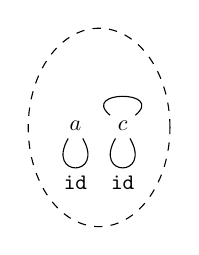
\begin{tikzpicture}[scale=0.6,every node/.style={scale=0.8}]
  \draw[dashed] (0,-0.3) ellipse (1.5cm and 2.1cm);
  \node[below] (A) at (-0.5,0) {$a$};
  \node[below] (C) at (0.5,0) {$c$};
  \path (A) edge [my loop] node[below] {\texttt{id}} (A);
  \path (C) edge [my loop] node[below] {\texttt{id}} (C);
  \path (C) edge [out=140, in=40, looseness=4] (C);
\end{tikzpicture}
\qquad \qquad \qquad
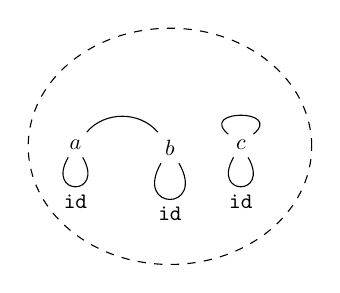
\begin{tikzpicture}[scale=0.6,every node/.style={scale=0.8}]
  \draw[dashed] (0,-0.3) ellipse (3cm and 2.5cm);
  \node[below] (A) at (-2,0) {$a$};
  \node[below] (B) at (0,0) {$b$};
  \node[below] (C) at (1.5,0) {$c$};
  \path (A) edge [bend left=50] (B);
  \path (C) edge [out=140, in=40, looseness=4] (C);
  \path (A) edge [my loop] node[below] {\texttt{id}} (A);
  \path (B) edge [my loop] node[below] {\texttt{id}} (B);
  \path (C) edge [my loop] node[below] {\texttt{id}} (C);
\end{tikzpicture}
\qquad \qquad \qquad
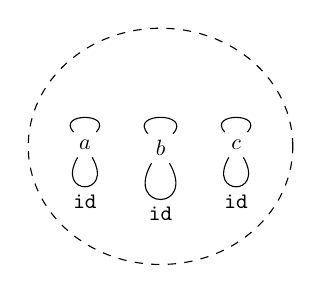
\begin{tikzpicture}[scale=0.6,every node/.style={scale=0.8}]
  \draw[dashed] (0,-0.3) ellipse (2.8cm and 2.5cm);
  \node[below] (A) at (-1.6,0) {$a$};
  \node[below] (B) at (0,0) {$b$};
  \node[below] (C) at (1.6,0) {$c$};
  \path (A) edge [my loop] node[below] {\texttt{id}} (A);
  \path (B) edge [my loop] node[below] {\texttt{id}} (B);
  \path (C) edge [my loop] node[below] {\texttt{id}} (C);
  \path (A) edge [loop above, looseness=3, in=48, out=132] (A);
  \path (B) edge [loop above, looseness=3, in=48, out=132] (B);
  \path (C) edge [loop above, looseness=3, in=48, out=132] (C);
\end{tikzpicture}
\end{center}
\caption{\label{fig:groupoids2}Example groupoids $G_1$, $G_2$, and $G_3$.}
\end{figure}

For plain sets, the definition just counts the elements as each element is its
own equivalence class and has exactly one automorphism (the identity). Without
quite formalizing them and relying on the informal diagrams until the next
section, we argue that each of the groupoids $G_1$, $G_2$, and $G_3$ in
Fig.~\ref{fig:groupoids2} has cardinality $\frac{3}{2}$. Groupoid~$G_1$ consists
of two isomorphism classes: class~$a$ has one object with one automorphism (the
identity) and class~$c$ has one object with two distinct automorphisms; the
cardinality is $\frac{1}{1} + \frac{1}{2} = \frac{3}{2}$. For groupoid~$G_2$, we
also have two isomorphism classes with representatives $a$ and $c$; the class
containing $a$ has two automorphisms starting from $a$: the identity and the
loop going from $a$ to~$b$ and back. By the groupoid axioms, this loop is
equivalent to the identity which means that the class containing $a$ has just
one automorphism. The isomorphism class of $c$ has two non-equivalent
automorphisms on it and hence the cardinality of $G_2$ is also
$\frac{1}{1} + \frac{1}{2} = \frac{3}{2}$. For~$G_3$, we have three isomorphism
classes, each with two non-equivalent automorphisms, and hence the cardinality
of $G_3$ is $\frac{1}{2} + \frac{1}{2} + \frac{1}{2} = \frac{3}{2}$.  It is
important to note that $G_1$ and $G_2$ are categorically equivalent groupoids,
but that $G_3$ is not categorically equivalent to either $G_1$ or $G_2$.  Roughly speaking
this is because the number of connected components is also a categorical
invariant of a groupoid, and here $G_1$ and $G_2$ have $2$ whilst $G_3$ has $3$.

%%%%%%%%%%%%%%%%%%%%%%%
\subsection{$\Pi$-Combinators as Automorphism Classes}

To formalize the counting above, we need, in the context of $\Pi$, a precise
definition of what it means for automorphisms to be ``distinct''. We start with
an example. Recall the type $\mathbb{3}$ with its three elements
$ll=\inl{\inl{\unitv}}$, $lr=\inl{\inr{\unitv}}$, and $r=\inr{\unitv}$. One of
the combinators of type $\mathbb{3} \iso \mathbb{3}$ is $\permtwo$. Observing
the results of applying the iterates $(\permtwo)^k$ for $k \in \Z$ on the three
elements we find:
\[\begin{array}{c@{\qquad\qquad}c}
\begin{array}{rcl}
\evalone{(\permtwo)^{2k}}{ll} &=& ll \\
\evalone{(\permtwo)^{2k}}{lr} &=& lr \\
\evalone{(\permtwo)^{2k}}{r} &=& r
\end{array} &
\begin{array}{rcl}
\evalone{(\permtwo)^{2k+1}}{ll} &=& lr \\
\evalone{(\permtwo)^{2k+1}}{lr} &=& ll \\
\evalone{(\permtwo)^{2k+1}}{r} &=& r
\end{array}
\end{array}\]
Furthermore, Lem.~\ref{lem:ordercancel} gives us the following families of
2-combinators $\alpha_{2k} : \idiso \isotwo (\permtwo)^{2k}$ and
$\alpha_{2k+1} : \permtwo \isotwo (\permtwo)^{2k+1}$. We can put these facts together to
construct a groupoid whose objects are the elements of $\mathbb{3}$, whose
1-morphisms relate $v_i$ and~$v_j$ if $\evalone{(\permtwo)^k}{v_i} = v_j$ for some
$k \in \Z$, and whose 2-morphisms are the families $\alpha_{2k}$ and
$\alpha_{2k+1}$ above. Such a construction produces the following groupoid where
each family of 1-morphisms that are identified by a family of 2-morphisms is
drawn using a thick line:

\begin{center}
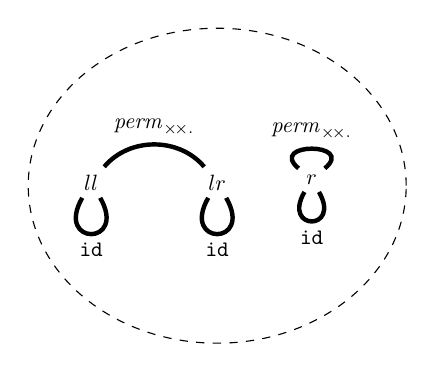
\begin{tikzpicture}[scale=0.8,every node/.style={scale=0.8}]
  \draw[dashed] (0,-0.3) ellipse (3cm and 2.5cm);
  \node[below] (A) at (-2,0) {$ll$};
  \node[below] (B) at (0,0) {$lr$};
  \node[below] (C) at (1.5,0) {$r$};
  \path[ultra  thick] (A) edge [bend left=50] node[above] {$\permtwo$} (B);
  \path[ultra  thick] (C) edge [out=140, in=40, looseness=4] node[above] {$\permtwo$}  (C);
  \path[ultra  thick] (A) edge [my loop] node[below] {\texttt{id}} (A);
  \path[ultra  thick] (B) edge [my loop] node[below] {\texttt{id}} (B);
  \path[ultra  thick] (C) edge [my loop] node[below] {\texttt{id}} (C);
\end{tikzpicture}
\end{center}

Clearly, the resulting groupoid is a reconstruction of $G_2$ in
Fig.~\ref{fig:groupoids2} using $\Pi$ types and combinators. As analyzed
earlier, this groupoid has cardinality $\frac{3}{2}$. From the perspective
of~$\Pi$, this cardinality corresponds to the number of elements in the
underlying set which is $3$ divided by the order of the combinator $\permtwo$
which is 2. It is important to note that, as Def.~\ref{def:order} states, the
calculation of the order of a 1-combinator is defined up to the equivalence
induced by 2-combinators.

%%%%%%%%%%%%%%%%%%%%%%%
\subsection{Iteration Groupoids $\order{p}$}

The previous construction known in the literature as an \emph{action
  groupoid}~\cite{groupoidintro} is quite useful: it allows us to take a set of
cardinality $N$ and a permutation on that set of order $P$ to construct a
groupoid of cardinality $\frac{N}{P}$. Although this idea allows us to construct
a groupoid of cardinality $\frac{3}{2}$ as shown above, it is not expressive
enough to construct a groupoid of cardinality, say, $\frac{1}{3}$. Indeed, if the
underlying set has only one element ($N=1$) the only permutation is the identity
and $P$ must be 1.

The construction, however, already contains the main ingredient needed for the construction of more general groupoids with fractional cardinality. This key piece is the set of iterates of a combinator which we formally define as follows.

\begin{definition}[$\iter{p}$]
For each 1-combinator $p : \tau\iso\tau$, we form the set $\iter{p}$ whose elements are triples consisting of an integer $k$, a 1-combinator $q : \tau\iso\tau$ and a 2-combinator $\alpha : q \isotwo p^k$.
\end{definition}
Each triple encodes our knowledge that we have some (arbitrary) iterate $q$ of $p$; we do not have any a priori knowledge of the actual syntactic structure of $q$, but we do know that it is equivalent to $p^k$. For example, we have:
\[\begin{array}{rcl}
 \iter{\permtwo} &=& \{ \triple{0}{\idiso}{\idisotwo},\triple{1}{\permtwo}{\idrdr}, \triple{-1}{\permtwo}{\idisotwo}, \ldots \}
\end{array}\]
The idea is that $\iter{\permtwo}$ is, up to equivalence, the set of all distinct iterates $(\permtwo)^k$ of $\permtwo$.  Because of the underlying group structure of automorphisms, there are, up to equivalence, only $\ord{\permtwo}$ distinct iterates in $\iter{\permtwo}$.  In a proof-irrelevant setting, $\iter{\permtwo}$ is simply $\{ \idiso, \permtwo \}$. In this section and the next, we will use the elements of $\iter{p}$ in two groupoid constructions as either objects (emphasizing their ``data'' aspect) or morphisms (emphasizing their ``symmetry'' aspect).

Given a 1-combinator $p : \tau\iso\tau$, we define the groupoid $\order{p}$ as
follows. The objects are the elements of $\iter{p}$, i.e., the triples
$\triple{k}{q}{\alpha}$ indexed by integers $k$, 1-combinators
$q : \tau\iso\tau$, and 2-combinators $\alpha : q \isotwo p^k$. We then add
(reversible) morphisms between any iterates related by 2-combinators;
categorically, this will make any such objects equivalent.  If $p$ has order
$o$, Lem.~\ref{lem:ordercancel} gives us a 2-combinator $\alpha$ which witnesses
that $p^i \isotwo p^{i+o}$.  Thus given two iterates $\triple{i}{q_i}{\alpha_i}$
and $\triple{i+o}{q_j}{\alpha_j}$, they must be equivalent since
$\alpha_i~\bullet~\alpha~\bullet~!\,\alpha_j$ shows that $q_i \isotwo q_j$.  In
other words $p^j$ will be equivalent to $p^k$ exactly when $j$ and $k$ differ by
$o$.  This informal description formalizes straightforwardly.

\begin{definition}[$\order{p}$] For each 1-combinator $p : \tau\iso\tau$, we form the groupoid $\order{p}$ as follows:
\begin{itemize}
\item objects are the elements $\triple{k}{q}{\alpha}$ of $\iter{p}$;
\item there is a morphism between $\triple{k_1}{q_1}{\alpha_1}$ and $\triple{k_2}{q_2}{\alpha_2}$ for each $\alpha : q_1 \isotwo q_2$
\end{itemize}
\end{definition}

Despite its involved internal structure, the groupoid $\order{p}$ is essentially
a set of cardinality $\ord{p}$.

\begin{lemma}
  $|\order{p}| = \ord{p}$
\end{lemma}
\begin{proof}
  Let $o = \ord{p}$. There are $o$ isomorphism classes of
  objects. Consider an object $x = \triple{k}{q}{\alpha}$, its
  isomorphism class $[x] = \triple{k+io}{q_i}{\alpha_i}$ where
  $i \in \Z$. The group $\textsf{Aut}(x)$ is the group generated by
  $\idisotwo$ and has order 1. Hence
  $|\order{p}| = \sum\limits_{1}^{o}\frac{1}{1} = o$.
\end{proof}

As an example, the groupoid $\order{(\permtwo)}$ can be represented as follows. Up to equivalence, this groupoid is indeed equivalent to a set with two elements $\idiso$ and $\permtwo$.

\begin{center}
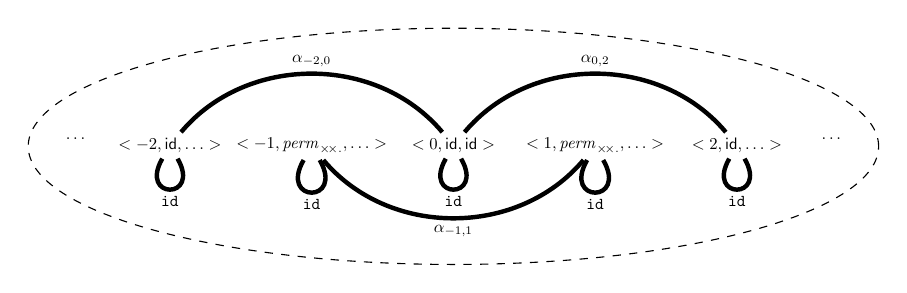
\begin{tikzpicture}[scale=0.6,every node/.style={scale=0.6}]
  \draw[dashed] (0,-0.3) ellipse (9cm and 2.5cm);

  \node[below] at (-8,0) {$\ldots$};
  \node[below] (A) at (-6,0) {$< -2 , \idiso , \ldots >$};
  \node[below] (B) at (-3,0) {$< -1 , \permtwo , \ldots >$};
  \node[below] (C) at (0,0) {$< 0, \idiso, \idisotwo >$};
  \node[below] (D) at (3,0) {$< 1 , \permtwo , \ldots >$};
  \node[below] (E) at (6,0) {$< 2 , \idiso , \ldots >$};
  \node[below] at (8,0) {$\ldots$};

  \path[ultra  thick] (A) edge [my loop] node[below] {\texttt{id}} (A);
  \path[ultra  thick] (B) edge [my loop] node[below] {\texttt{id}} (B);
  \path[ultra  thick] (C) edge [my loop] node[below] {\texttt{id}} (C);
  \path[ultra  thick] (D) edge [my loop] node[below] {\texttt{id}} (D);
  \path[ultra  thick] (E) edge [my loop] node[below] {\texttt{id}} (E);

  \path[ultra  thick] (A) edge [bend left=50] node[above] {$\alpha_{-2,0}$} (C);
  \path[ultra  thick] (C) edge [bend left=50] node[above] {$\alpha_{0,2}$} (E);
  \path[ultra  thick] (B) edge [bend left=-50] node[below] {$\alpha_{-1,1}$} (D);

\end{tikzpicture}
\end{center}

%%%%%%%%%%%%%%%%%%%%%%%
\subsection{Symmetry Groupoids $\iorder{p}$}\label{sec:symmetryg}

The elements of $\iter{p}$ form a group under the following operation:
\[
\triple{k_1}{p_1}{\alpha_1} ~\circ~ \triple{k_2}{p_2}{\alpha_2} =
 \triple{k_1+k_2}{p_1 \odot p_2}{(\alpha_1 ~\respstwo~
    \alpha_2)~\transtwo~(\distiterplus{p}{k_1}{k_2})}
\]
where $\distiterplus{p}{k_1}{k_2}$ is defined in
Lem.~\ref{lem:distiterplus}. The common categorical representation of a group is
a category with one trivial object and the group elements as morphisms on that
trivial object. Our construction of the groupoid $\iorder{p}$ is essentially the
same.

\begin{definition}[$\iorder{p}$] For each 1-combinator $p : \tau\iso\tau$, we form the 2-groupoid $\iorder{p}$ as follows:
\begin{itemize}
\item the objects are the iterates of the identity combinator on $\tau$;
\item the morphisms between every pair of objects are the elements of $\iter{p}$;
\item there is a 2-morphism between 1-morphisms $\triple{k_1}{q_1}{\alpha_1}$ and $\triple{k_2}{q_2}{\alpha_2}$ for every $\alpha : q_1 \isotwo q_2$.
\end{itemize}
\end{definition}

Note that for each power $p ^ i$ of $p$, there is a morphism
$\triple{k}{q}{\alpha}$ in $\iter{p}$ such that $q$ annihilates $p^i$ to the
identity.

\paragraph*{Remark.} Note also that everything is well-defined even if we choose
$p : \zt\iso\zt$. In that case, the cardinality is 1.

\begin{lemma}
  $|\iorder{p}| = \frac{1}{\ord{p}}$
\end{lemma}
\begin{proof}
  Let $o = \ord{p}$. The objects form one isomorphism class
  $[p]$. There are, up to equivalence, exactly $\ord{p}$ distinct
  morphisms on this equivalence class. Hence, the group
  $\textsf{Aut}([p])$ is the group generated by
  $p^0, p^1 \dots p^{o-1}$, and the cardinality $|\iorder{p}|$ is
  $\frac{1}{o}$.
\end{proof}

As an example, the groupoid $\iorder{(\permtwo)}$ can be represented as follows.

\begin{center}
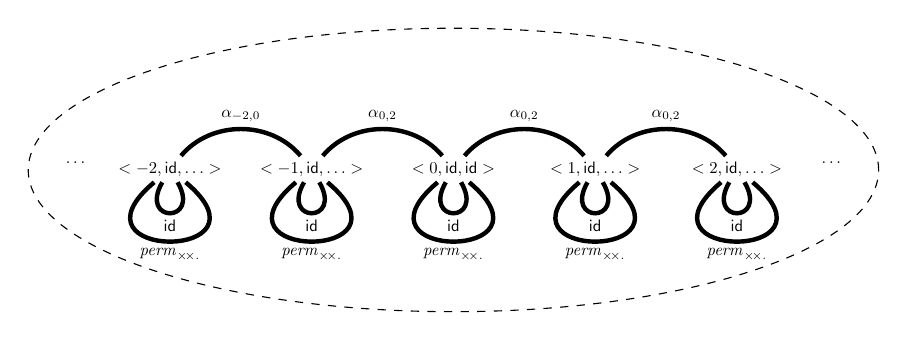
\begin{tikzpicture}[scale=0.6,every node/.style={scale=0.6}]
  \draw[dashed] (0,-0.3) ellipse (9cm and 3cm);

  \node[below] at (-8,0) {$\ldots$};
  \node[below] (A) at (-6,0) {$< -2 , \idiso , \ldots >$};
  \node[below] (B) at (-3,0) {$< -1 , \idiso , \ldots >$};
  \node[below] (C) at (0,0) {$< 0, \idiso, \idisotwo >$};
  \node[below] (D) at (3,0) {$< 1 , \idiso , \ldots >$};
  \node[below] (E) at (6,0) {$< 2 , \idiso , \ldots >$};
  \node[below] at (8,0) {$\ldots$};

  \path[ultra  thick] (A) edge [my loop] node[below] {$\idiso$} (A);
  \path[ultra  thick] (B) edge [my loop] node[below] {$\idiso$} (B);
  \path[ultra  thick] (C) edge [my loop] node[below] {$\idiso$} (C);
  \path[ultra  thick] (D) edge [my loop] node[below] {$\idiso$} (D);
  \path[ultra  thick] (E) edge [my loop] node[below] {$\idiso$} (E);

  \path[ultra  thick] (A) edge [bend left=50] node[above] {$\alpha_{-2,0}$} (B);
  \path[ultra  thick] (B) edge [bend left=50] node[above] {$\alpha_{0,2}$} (C);
  \path[ultra  thick] (C) edge [bend left=50] node[above] {$\alpha_{0,2}$} (D);
  \path[ultra  thick] (D) edge [bend left=50] node[above] {$\alpha_{0,2}$} (E);

  \path[ultra  thick] (A) edge [out=-140, in=-40, looseness=10] node[below] {$\permtwo$} (A);
  \path[ultra  thick] (B) edge [out=-140, in=-40, looseness=10] node[below] {$\permtwo$} (B);
  \path[ultra  thick] (C) edge [out=-140, in=-40, looseness=10] node[below] {$\permtwo$} (C);
  \path[ultra  thick] (D) edge [out=-140, in=-40, looseness=10] node[below] {$\permtwo$} (D);
  \path[ultra  thick] (E) edge [out=-140, in=-40, looseness=10] node[below] {$\permtwo$} (E);
\end{tikzpicture}
\end{center}

%%%%%%%%%%%%%%%%%%%%%%%
\subsection{Looping and Delooping}

Our constructions of $\order{p}$ and $\iorder{p}$ are instances of a general
pattern that we have instantiated to the setting of $\Pi$ and adapted to
explicitly refer to weak (i.e., up to $\isotwo$ in our case) equivalences. In
the general construction~\cite{looping}, a group $G$ is known to induce two
groupoids, a looping groupoid $\looping{G}$ and a delooping groupoid
$\delooping{G}$. These are defined as follows.

The looping groupoid $\looping{G}$ has the elements $g$ of the group $G$ as
objects and morphisms between elements in the same conjugacy class; that is,
there is a
morphism between elements~$g$ and $h$ iff there exists an $x \in G$ such that
$h = x^{-1} \cdot g \cdot x$. Fixing a type $\tau$ and a particular 1-combinator
$p : \tau \iso \tau$, we get a group whose elements are the iterates $p^k$. The
corresponding looping groupoid has all the iterates as objects, and morphisms
between $p^{k_1}$ and $p^{k_2}$ whenever there exists an integer $j$ such that
$p^{k_2}$ is equivalent to $p^{-j} \odot p^{k_1} \odot p^{j}$. By
Lem.~\ref{lem:distiterplus}, the latter term is $\isotwo$-equivalent to
$p^{-j+k_1+j}$ which is $\isotwo$-equivalent to $p^{k_1}$. In other words, we
have a morphism between $p^{k_1}$ and $p^{k_2}$ whenever they are
$\isotwo$-equivalent which is consistent with our definition of iteration
groupoids.

The delooping groupoid $\delooping{G}$ has one trivial element $\ast$, and for
each group element $g$ a morphism (loop) from $\ast$ to $\ast$. Modulo
$\isotwo$-equivalences, this is consistent with our definition of symmetry
groupoids.

%%%%%%%%%%%%%%%%%%%%%%%
\subsection{Products of Iteration and Symmetry Groupoids}
\label{sub:products}

If we are to build a compositional programming language around iteration and
symmetry groupoids, we need to ensure that they compose sensibly with the
existing type formers. Groupoids, viewed as categories, come associated with
natural notions of sums and products, and one might expect or hope that
identities which hold for rational numbers lift to identities in our
situation. The integration of these groupoids with the categorical sum is
complicated and left for future work. For products, the most prominent identity,
from which many other identities follow, is:
\[
\order{p} \circledast \iorder{p} \simeq \order{\idiso}
\]
The left hand side is the categorical product of the iteration groupoid and
symmetry groupoid for some arbitrary 1-combinator $p$. The cardinality of this
groupoid is 1. The right hand side is the iteration groupoid for the identity
1-combinator which also has cardinality 1. The groupoids on either side are
however not isomorphic, there do not exist full and faithful functors between
them, and hence $\simeq$ cannot be categorical equivalence.

There are however weaker notions of groupoid equivalence, such as \emph{Morita
  equivalence}~\cite{looping}\cite[C5.3]{johnstone2002sketches}, that identify
the two groupoids above.  Although the notion of equivalence we use in the next
section appears novel, it is related ``in spirit'' to Morita equivalence and we
find it useful to give a small example. We will verify that the product of the
groupoid $\order{\permfive}$ of cardinality 3 and the groupoid
$\iorder{\permfive}$ of cardinality $\frac{1}{3}$ is Morita equivalent to the
trivial groupoid with only one distinct object and one trivial automorphism. To
avoid clutter, we assume the groupoids are strict, e.g., that the groupoid
$\order{\permfive}$ has three elements (instead of 3 isomorphism classes of
elements).

Getting an equivalence in this case reduces to finding a \emph{Morita morphism}
from $\order{\idiso}$ to $\order{\permfive} \circledast
\iorder{\permfive}$.
This is a functor $\psi$ from the unit groupoid to the product groupoid, say
$G$, with an additional condition that the commutative diagram below is a
\emph{pullback}, where $s,t$ are the \emph{source} and \emph{target} maps, and
$\ot$, $\mathbb{3}$ are the $1$- and $3$-point discrete groupoids defined
previously.

\begin{center}
\begin{tikzcd}
    Q
    \arrow[drr, bend left, "{\xi_1}"]
    \arrow[ddr, bend right, "{(s,t)}"]
    \arrow[dr, dotted] & & \\
    & \order{\idiso} \arrow[r, "{\psi_1}"] \arrow[d, "{(s,t)}"]
    & G \arrow[d, "{(s,t)}"] \\
    & \ot \times \ot \arrow[r, "{\psi_0 \times \psi_0}"]
    & \mathbb{3} \times \mathbb{3}
\end{tikzcd}
\end{center}

\medskip\noindent The intuition is that the codomain consists of three objects
with associated morphisms, each of them counting as a ``third.'' The functor
from $\order{\idiso}$ to $\order{\permfive} \circledast \iorder{\permfive}$ must
include an arbitrary choice of ``which third'' to target and the universality
condition of the pullback ensures that the choice is ultimately insignificant as
it leads to the same result as every other possible functor.

To summarize, the equivalence between the two groupoids requires a \emph{local}
map that chooses a target and a \emph{global} condition ensuring that the choice
ultimately annihilates. The challenge we aim to solve in the next section is to
turn this idea into an operational semantics that somehow combines the local and
global aspects of the equivalence. We will be inspired by the folklore result in
the categorical semantics of dependent type theory~\cite{subpullback}, first
explained by Paul Taylor~\cite{practicalfoundations}, that ``substitution into a
dependent type is a pullback''.

%%%%%%%%%%%%%%%%%%%%%%%%%%%%%%%%%%%%%%%%%%%%%%%%%%%%%%%%%%%%%%%%%%%%%%%%%%%%%%
\section{$\Pi^/$: Syntax and Semantics}

We are now ready to turn the groupoid constructions from the previous section
into an extension of $\Pi$ with new type constructors and combinators for
creating and manipulating syntactic counterparts to $\order{p}$ and
$\iorder{p}$.  Just adding the ``obvious'' types and combinators does
not work; however, as the failures are quite informative, we nevertheless go
through this first attempt.  This will help illustrate why we need extra
machinery in Sec.~\ref{sec:deppointedtypes}.

\begin{figure}[t]
\[\begin{array}{rrcll}
\unitetl/ :&  \order{\idiso} \circledast \mathbb{T} & \leftrightspoon & \mathbb{T} &: \unititl/ \\
\unitetr/ :&  \mathbb{T} \circledast \order{\idiso} & \leftrightspoon & \mathbb{T} &: \unititr/ \\
\swapt/ :&  \mathbb{T}_1 \circledast \mathbb{T}_2 & \leftrightspoon & \mathbb{T}_2 \circledast \mathbb{T}_1 &: \swapt/ \\
\assoclt/ :&  \mathbb{T}_1 \circledast (\mathbb{T}_2 \circledast \mathbb{T}_3) & \leftrightspoon & (\mathbb{T}_1 \circledast \mathbb{T}_2) \circledast \mathbb{T}_3
  &: \assocrt/ \\
\\
\eta- :& \order{\idiso} & \leftrightspoon & \iorder{c} \circledast \order{c} &: \epsilon- \\
\eta+ :& \order{\idiso} & \leftrightspoon & \order{c} \circledast \iorder{c} &: \epsilon+ \\
\end{array}\]

\[\begin{array}{c}
\Rule{}
{}
{\jdg{}{}{\idiso/ : \mathbb{T} \leftrightspoon \mathbb{T}}}
{}
\qquad
\Rule{}
{\jdg{}{}{\rho_1 : \mathbb{T}_1 \leftrightspoon \mathbb{T}_2} \quad \rho_2 : \mathbb{T}_2 \leftrightspoon \mathbb{T}_3}
{\jdg{}{}{\rho_1 \circledcirc \rho_2 : \mathbb{T}_1 \leftrightspoon \mathbb{T}_3}}
{}
\\
\\
\Rule{}
{\jdg{}{}{\alpha : c_1 \isotwo c_2}}
{\jdg{}{}{\order{\alpha} : \order{c_1}  \leftrightspoon \order{c_2}}}
{}
\qquad
\Rule{}
{\jdg{}{}{\rho_1 : \mathbb{T}_1 \leftrightspoon \mathbb{T}_2} \quad \rho_2 : \mathbb{T}_3 \leftrightspoon \mathbb{T}_4}
{\jdg{}{}{\rho_1 \circledast \rho_2 : \mathbb{T}_1 \circledast \mathbb{T}_3 \leftrightspoon \mathbb{T}_2 \circledast \mathbb{T}_4}}
{}
\end{array}\]

Each combinator $\rho$ has an inverse.
\caption{$\Pi^/$ fractional combinators (non-dependent version)}
\label{pifrac:comb}
\end{figure}

%%%%%
\subsection{First attempt: non-dependent version}

As a first approximation to the language we seek, we consider adding three new
syntactic categories to the definition of $\Pi$ in Sec.~\ref{opsempi}:

\begin{definition}[Non-dependent $\Pi^/$]
\label{def:pifrac}
The syntax of (non-dependent) $\Pi^/$ is given by the following categories:
\[\begin{array}{lrcl}
(\textrm{Types}) & \tau &::=& [\textit{see Def.~\ref{def:pi}}] \\
(\textrm{Values}) & v &::=& [\textit{see Def.~\ref{def:pi}}] \\
(\textrm{1-combinators}) & c &:& \tau_1 \iso \tau_2 ~::= [\textit{see Def.~\ref{def:pi}}] \\
(\textrm{2-combinators}) & \alpha &:& c_1 \isotwo c_2 \mbox{~where~}
  c_1, c_2 : \tau_1 \iso \tau_2 ~::= [\textit{see Def.~\ref{def:pi}}] \\
\\
(\textrm{Fractional Types}) & \mathbb{T} &::=&
  \order{c} \alt \iorder{c} \alt \mathbb{T}_1 \circledast \mathbb{T}_2 \\
 (\textrm{Fractional Values}) & \mathbb{V} &::=&
  c^k \alt 1/c^k \alt \langle \mathbb{V},\mathbb{V} \rangle \\
 (\textrm{/-combinators}) & \rho &:& \mathbb{T}_1 \leftrightspoon \mathbb{T}_2 ~::=
  [\textit{see Fig.~\ref{pifrac:comb}}]
\end{array}\]
\end{definition}

The syntactic category $\ft$ of fractional types introduces type expressions
for iteration groupoids, symmetry groupoids, and their products. The
combinators that relate these fractional types are in Fig.~\ref{pifrac:comb}.
The bottom group includes identity and sequential composition~$\circledcirc$
combinators and ensures that the combinators can be applied anywhere inside a
product $\circledast$. There is also a combinator that relates two types
$\order{c_1}$ and $\order{c_2}$ via $\order{\alpha}$ whenever $\alpha : c_1
\isotwo c_2$.  Indeed if $c_1$ and $c_2$ are considered equivalent via a
$2$-combinator then we also consider their iteration groupoids to be equivalent.
The top group ensures that $\circledast$ carries a symmetric monoidal structure
with combinators witnessing the unit, commutativity, and associativity
properties. The last two pairs of combinators $\eta\!- / \epsilon-$ and
$\eta\!+ / \epsilon+$ are inspired from the definition of compact closed
categories~\cite{ccc} which are symmetric monoidal categories in which every
object has a dual. They are the ones that witness the ``fractional'' nature of
symmetry groupoids as motivated in Sec.~\ref{sub:products}.

The last new syntactic category in $\Pi^/$ is that of values which deserves some
additional discussion. When types denote sets, values of a type are clear: they
are just the elements of the set.  In the case when types are groupoids, this is
less clear, especially when the groupoid cardinality is a proper fraction.  What
we get instead are equivalence classes of values.  The idea is not uncommon: in
the conventional $\lambda$-calculus, we list $\lambda x.x$ and $\lambda y.y$ as
separate values of type $\tau \rightarrow \tau$ and then provide a separate
equivalence relation ($\alpha$-equivalence) to express the fact that these two
values are indistinguishable. The treatment in our setting is similar: for
iteration groupoids $\order{c}$, every distinct iterate $c^k$ is listed as a
separate value with the understanding that some iterates are
$\isotwo$-equivalent. Similarly for symmetry groupoids $\iorder{c}$, every
morphism is listed as a value $1/c^k$ with the same understanding that some of
these morphisms are $\isotwo$-equivalent.

To understand the challenge in designing an operational semantics for $\eta$ and
$\epsilon$ in the non-dependent setting, we consider the ``zigzag'' circuit in
Fig.~\ref{fig:zigzag}. Algebraically this circuit corresponds to the following
manipulation on types:
\[
x \mapsto (1 \times x) \mapsto ((x \times 1/x) \times x)
\mapsto (x \times (1/x \times x)) \mapsto (x \times 1) \mapsto x
\]
and by the coherence conditions of compact closed categories, we expect this
circuit, when run in either direction, to be equivalent to the
identity. Consider now the case of a combinator $c$ whose order is greater than
or equal to 2, i.e., the type $\order{c}$ has at least two distinct values
$\idiso$ and $c$ and the type $\iorder{c}$ has at least two distinct values
$1/\idiso$ and $1/c$. We require this circuit to produce $\idiso$ when given
$\idiso$ from either end, and similarly to produce $c$ when given $c$ from
either end. The problem becomes apparent when one observes that the uses of
$\eta+$ in the left-to-right execution and the use of $\epsilon-$ in the
right-to-left execution must behave differently depending on the incoming
value. But the ``local'' information available to either of these combinators
does not include the ``global'' information about the incoming value and there
is no way for them to make consistent guesses locally. It is possible to design
an operational semantics that uses computational effects to enable spatially
separated parts of the program to communicate in a way that is reminiscent of
entanglement in quantum mechanics. Possibilities to realize this communication
are global reference cells, backtracking, and logical variables with
unification. We choose however to present in the next section a more abstract
approach that encodes the required dependency in dataflow constraints using
dependent types.

\begin{figure}[t]
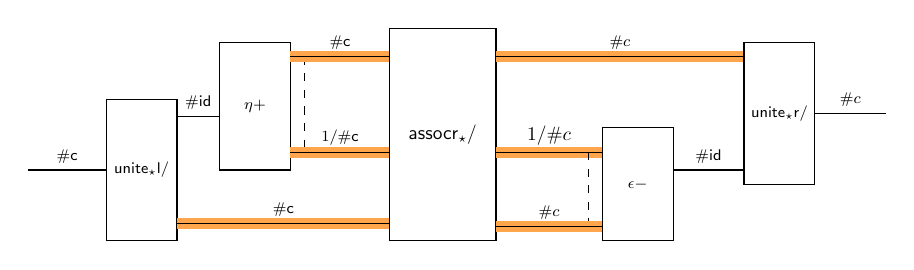
\begin{tikzpicture}[scale=0.9,every node/.style={scale=0.7},highlight/.style={line width=4pt,orange!70}]
  \draw (0,0) -- (1,0) -- (1,2) -- (0,2) -- cycle;
  \node at (0.5,1) {\footnotesize{$\unitetl/$}};
  \path (-1.1,1) edge node[above] {\footnotesize{${\textsf{\#c}}$}} (0,1);
  \path (1,1.75) edge node[above] {\footnotesize{$\order{\idiso}$}} (1.6,1.75);
  \path [highlight] (1,0.25) edge node[above] {} (4,0.25);
  \path (1,0.25) edge node[above] {\footnotesize{${\textsf{\#c}}$}} (4,0.25);
  \draw (1.6,1) -- (2.6,1) -- (2.6,2.8) -- (1.6,2.8) -- cycle;
  \node at (2.1,1.9) {\footnotesize{$\eta+$}};
  \draw[dashed] (2.8,2.6) -- (2.8,1.25);
  \path [highlight] (2.6,2.6) edge node[above] {} (4,2.6);
  \path (2.6,2.6) edge node[above] {\footnotesize{${\textsf{\#c}}$}} (4,2.6);
  \path [highlight] (2.6,1.25) edge node[above] {} (4,1.25);
  \path (2.6,1.25) edge node[above] {\footnotesize{$1/\textsf{\#c}$}} (4,1.25);
  \draw (4,0) -- (5.5,0) -- (5.5,3) -- (4,3) -- cycle;
  \node at (4.75,1.5) {$\footnotesize{\assocrt/}$};
  \path [highlight] (5.5,1.25) edge node[above] {} (7,1.25);
  \path (5.5,1.25) edge node[above] {$\footnotesize{1/\#c}$} (7,1.25);
  \path [highlight] (5.5,2.6) edge node[above] {} (9,2.6);
  \path (5.5,2.6) edge node[above] {\footnotesize{$\#c$}} (9,2.6);
  \draw (7,0) -- (8,0) -- (8,1.6) -- (7,1.6) -- cycle;
  \node at (7.5,0.8) {\footnotesize{$\epsilon-$}};
  \draw[dashed] (6.8,0.2) -- (6.8,1.25);
  \path (8,1) edge node[above] {\footnotesize{$\order{\idiso}$}} (9,1);
  \path [highlight] (5.5,0.2) edge node[above] {} (7,0.2);
  \path (5.5,0.2) edge node[above] {\footnotesize{$\#c$}} (7,0.2);
  \draw (9,0.8) -- (10,0.8) -- (10,2.8) -- (9,2.8) -- cycle;
  \node at (9.5,1.8) {\footnotesize{$\unitetr/$}};
  \path (10,1.8) edge node [above] {\footnotesize{$\#c$}} (11,1.8);
\end{tikzpicture}
\caption{\label{fig:zigzag} Zigzag}
\end{figure}

\begin{figure}[t]
{\footnotesize
\[\begin{array}{rrcll}
\unitetl/ :& \forall\exists{\overline{k}}.[\order{\idiso} \circledast \mathbb{T},
                                                   \langle \idiso,v \rangle]
  & \leftrightblackspoon &
                   \forall\exists{\overline{k}}.[\mathbb{T},v]
  &: \unititl/ \\
\unitetr/ :& \forall\exists{\overline{k}}.[\mathbb{T} \circledast \order{\idiso},
                                                    \langle v,\idiso]
  & \leftrightblackspoon &
                   \forall\exists{\overline{k}}.[\mathbb{T},v]
  &: \unititr/ \\
\swapt/ :& \forall\exists{\overline{k}}.[\mathbb{T}_1 \circledast \mathbb{T}_2,
                                                   \langle v_1,v_2 \rangle]
 & \leftrightblackspoon &
                  \forall\exists{\overline{k}}.[\mathbb{T}_2 \circledast \mathbb{T}_1,
                                                  \langle v_2,v_1 \rangle]
  &: \swapt/ \\
  \assoclt/ :& \forall\exists{\overline{k}}.
               [\mathbb{T}_1 \circledast (\mathbb{T}_2 \circledast \mathbb{T}_3),
                                        \langle v_1,\langle v_2,v_3 \rangle]
  & \leftrightblackspoon &
                      \forall\exists{\overline{k}}.
               [(\mathbb{T}_1 \circledast \mathbb{T}_2) \circledast \mathbb{T}_3,
                                       \langle \langle v_1,v_2 \rangle , v_3 \rangle]
  &: \assocrt/ \\
\\
\eta- :& [\order{\idiso},\idiso] & \leftrightblackspoon &
  \forall\exists{k}.[\iorder{c} \circledast \order{c}, \langle 1/c^k, c^k  \rangle]
  & : \epsilon- \\
\eta+ :& [\order{\idiso},\idiso] & \leftrightblackspoon &
  \forall\exists{k}.[\order{c} \circledast \iorder{c}, \langle c^k,1/c^k \rangle]
  & : \epsilon+ \\
\synchl :& \forall\exists{k}.[(\order{c}\circledast\iorder{c})\circledast\order{c},
  \langle \langle c^k,1/c^k \rangle, c^i]
  & \leftrightblackspoon &
  [(\order{c}\circledast\iorder{c})\circledast\order{c},
    \langle \langle c^i,1/c^i \rangle, c^i]
  & : \packl \\
\synchr :& \forall\exists{k}.[\order{c}\circledast(\iorder{c}\circledast\order{c}),
  \langle c^i, \langle 1/c^k, c^k \rangle \rangle]
  & \leftrightblackspoon &
   [\order{c}\circledast(\iorder{c}\circledast\order{c}),
   \langle c^i, \langle 1/c^i, c^i \rangle \rangle]
  & : \packr
\end{array}\]
\[\begin{array}{c}
\Rule{}
{}
{\jdg{}{}{\idiso/ : \forall\exists{\overline{k}}.[\mathbb{T},v] \leftrightblackspoon
   \forall\exists{\overline{k}}.[\mathbb{T},v]}}
{}
~~
\Rule{}
{\jdg{}{}{\alpha : c_1 \isotwo c_2}}
{\jdg{}{}{(\order{\alpha})_k :
 [\order{c_1},c_1^k]  \leftrightblackspoon
 [\order{c_2},c_2^k]}}
{}
\\
\\
\Rule{}
{\jdg{}{}{\rho_1 :
  \forall\exists{\overline{k_1}}.[\mathbb{T}_1,v_1] \leftrightblackspoon
  \forall\exists{\overline{k_2}}.[\mathbb{T}_2,v_2]} \quad
  \rho_2 :
  \forall\exists{\overline{k_2}}.[\mathbb{T}_2,v_2] \leftrightblackspoon
  \forall\exists{\overline{k_3}}.[\mathbb{T}_3,v_3]}
{\jdg{}{}{\rho_1 \circledcirc \rho_2 :
 \forall\exists{\overline{k_1}}.[\mathbb{T}_1,v_1] \leftrightblackspoon
 \forall\exists{\overline{k_3}}.[\mathbb{T}_3},v_3]}
{}
\\
\\
\Rule{}
{\jdg{}{}{\rho_1 :
 \forall\exists{\overline{k_1}}.[\mathbb{T}_1,v_1] \leftrightblackspoon
 \forall\exists{\overline{k_2}}.[\mathbb{T}_2,v_2]}
 \qquad \rho_2 :
 \forall\exists{\overline{k_3}}.[\mathbb{T}_3,v_3] \leftrightblackspoon
 \forall\exists{\overline{k_4}}.[\mathbb{T}_4,v_4]}
{\jdg{}{}{\rho_1 \circledast \rho_2 :
  \forall\exists{\overline{k_1k_3}}.[\mathbb{T}_1 \circledast \mathbb{T}_3, \langle v_1,v_3 \rangle]
  \leftrightblackspoon
  \forall\exists{\overline{k_2k_4}}.[\mathbb{T}_2 \circledast \mathbb{T}_4}, \langle v_2,v_4 \rangle]}
{}
\end{array}\]
\\
Each combinator $\rho_\bullet$ has an inverse $\rho_\bullet^{-1}$.
A rule $\mathbb{T_1}_\bullet \leftrightblackspoon
\forall\exists{k}.\mathbb{T_2}_\bullet$ introduces a $\forall$ in the left-to-right
direction and eliminates an $\exists$ in the right-to-left direction. A rule
$\forall\exists{k}.\mathbb{T_1}_\bullet \leftrightblackspoon
\mathbb{T_2}_\bullet$ eliminates a $\forall$ in the left-to-right direction and
introduces an $\exists$ in the right-to-left direction. A rule
$\forall\exists{k}.\mathbb{T_1}_\bullet \leftrightblackspoon
\forall\exists{k}.\mathbb{T_2}_\bullet$ maintains (think of elimination then
introduction) the universal quantifier in the left-to-right direction and
the existential quantifier in the right-to-left direction. We omit the
quantifiers when the sequence of bound variables is empty.
}
\caption{$\Pi^/$ fractional combinators (dependent version)}
\label{pifracd:comb}
\end{figure}

%%%%%
\subsection{Dependent Pointed Types}\label{sec:deppointedtypes}

We modify the syntax of $\Pi^/$ as follows.

\begin{definition}[Dependent $\Pi^/$]
\label{def:pifracd}
The syntax of dependent $\Pi^/$ differs from Def.~\ref{def:pifrac} as follows:
\[\begin{array}{lrcl}
(\textrm{Fractional Types}) & \mathbb{T_\bullet} &::=&
  [\order{c},c^k] \alt
  [\iorder{c},1/c^k] \alt
  [\mathbb{T}_1 \circledast \mathbb{T}_2,\langle v_1,v_2 \rangle] \alt
  \forall k.\mathbb{T_\bullet} \alt \exists k.\mathbb{T_\bullet} \\
 (\textrm{/-combinators}) & \rho_\bullet &:&
  \mathbb{T_1}_{\bullet} \leftrightblackspoon \mathbb{T_2}_{\bullet} ~::=
  [\textit{see Fig.~\ref{pifracd:comb}}]
\end{array}\]
\end{definition}

In the new definition, we enrich the types to pointed types $\mathbb{T_\bullet}$
where each type $\mathbb{T}$ refers to a particular value $v$ in
$\mathbb{T}$. As all fractional types are inhabited (see Remark in
Sec.~\ref{sec:symmetryg}), there is no loss in generality in going to pointed
types. We then allow universal quantification over indices $k$ associated to
values, over a collection of types.  In particular, the type
$\forall k.[\order{c} \circledast \iorder{c}, \langle c^k, 1/c^k \rangle]$
imposes a constraint on the two values associated with the types $\order{c}$ and
$\iorder{c}$; they must be ``synchronized'' by sharing the same~$k$ but are
otherwise arbitrary. Once we introduce a universal quantifier in one direction
of execution, we are led to also include an existential quantifier for the
reverse execution. Intuitively, a forward evaluation step that is at liberty to
choose a $k$ will, when reversed encounter a particular, i.e., existentially
quantified, $k$. A type $\mathbb{T}_\bullet$ is therefore generally of the form
$\forall\exists{\overline{k}}.[\mathbb{T},v]$ where all the quantifiers are
lifted to the top followed by a non-dependent type and a value in that type.

The adaptation of the combinators to the pointed dependent setting in Fig .~\ref
{pifracd:comb} is relatively straightforward. First, the types of the
combinators must keep track of how the value currently in focus changes during
evaluation, and hence directly encode the operational semantics of the
language. As suggested above, the quantifiers are interpreted differently
depending on which direction the rule is used. We use a $\forall\exists$
notation to express the presence of \emph{one} quantifier that is interpreted
differently in each direction. The notation has the advantage of being compact,
avoiding duplication, and making the symmetry of the rules explicit. We also
include two new pairs of combinators $\synchl/\packl$ and $\synchr/\packr$ that
serve as explicit quantifier introduction and elimination rules: they serve as
explicit ``synchronization'' points as illustrated in the example below.

The example revisits the zigzag circuit in Fig.~\ref{fig:zigzag} using the
dependent types and the new explicit synchronization primitives. The evaluation
proceeds as follows where we disambiguate the uses of $\forall$ and $\exists$
in each direction for clarity:

\paragraph*{Forward execution of zigzag circuit with synchronization.}
\[\begin{array}{rcl}
[\order{c},c^i]
&\stackrel{\unitetl/}{\leftrightblackspoon}&
  [\order{id}\circledast\order{c}, \langle \idiso,c^i \rangle] \\
&\stackrel{\eta+\circledast\idiso/}{\leftrightblackspoon}&
  \forall{k}.[(\order{c}\circledast\iorder{c})\circledast\order{c},
  \langle \langle c^k,1/c^k \rangle,c^i \rangle] \\
&\stackrel{\synchl}{\leftrightblackspoon}&
  [\langle \langle c^i,1/c^i \rangle,c^i \rangle] \\
&\stackrel{\assocrt/}{\leftrightblackspoon}&
  [\order{c}\circledast(\iorder{c}\circledast\order{c}),
  \langle c^i, \langle 1/c^i,c^i \rangle\rangle] \\
&\stackrel{\packr}{\leftrightblackspoon}&
  \exists{k}.[\order{c}\circledast(\iorder{c}\circledast\order{c}),
  \langle c^i, \langle 1/c^k,c^k \rangle\rangle] \\
&\stackrel{\idiso/\circledast\epsilon-}{\leftrightblackspoon}&
  [\order{c}\circledast\order{\idiso},
  \langle c^i, \idiso \rangle] \\
&\stackrel{\unitetr/}{\leftrightblackspoon}&
  [\order{c}, c^i]
\end{array}\]

\paragraph*{Reverse execution of zigzag circuit with synchronization.}
\[\begin{array}{rcl}
  [\order{c}, c^i]
&\stackrel{\unitetr/}{\leftrightblackspoon}&
  [\order{c}\circledast\order{\idiso},
  \langle c^i, \idiso \rangle] \\
&\stackrel{\idiso/\circledast\epsilon-}{\leftrightblackspoon}&
  \forall{k}.[\order{c}\circledast(\iorder{c}\circledast\order{c}),
  \langle c^i, \langle 1/c^k,c^k \rangle\rangle] \\
&\stackrel{\synchr}{\leftrightblackspoon}&
 [(\order{c}\circledast\iorder{c})\circledast\order{c},
  \langle \langle c^i,1/c^i \rangle,c^i \rangle] \\
&\stackrel{\assocrt/}{\leftrightblackspoon}&
  [(\order{c}\circledast\iorder{c})\circledast\order{c},
  \langle \langle c^i,1/c^i \rangle,c^i \rangle] \\
&\stackrel{\packl}{\leftrightblackspoon}&
  \exists{k}.[(\order{c}\circledast\iorder{c})\circledast\order{c},
  \langle \langle c^k,1/c^k \rangle,c^i \rangle] \\
&\stackrel{\eta+\circledast\idiso/}{\leftrightblackspoon}&
  [\order{\idiso}\circledast\order{c}, \langle \idiso,c^i\rangle] \\
&\stackrel{\unitetl/}{\leftrightblackspoon}&
  [\order{c},c^i]
\end{array}\]

%%%%
\subsection{Additional Examples}

Compact closed categories support various interesting
constructions~\cite{abramsky-2008}, such as duals, name and coname, and
trace~\cite{joyal1996traced,Hasegawa:1997:RCS:645893.671607}, which eventually
lead to a certain notion of recursive higher-order functions. These
constructions do not immediately transfer to the context of $\Pi^/$ as we have
explicit quantifiers and synchronization primitives that are not present in the
conventional setting. Resolving these subtleties will provide the first
operational interpretation known to us of multiplicative higher-order recursive
functions.

% \begin{figure}[htb]
%   \centering
%   \begin{tikzpicture}[scale=0.9,every node/.style={scale=0.7},highlight/.style={line width=4pt,orange!70}]
%     \path [highlight] (-1,1) edge node[above] {} (0,1);
%     \path (-1,1) edge node[above] {\footnotesize{$1/{\textsf{\#d}}$}} (0,1);

%     \draw (0,0) -- (1,0) -- (1,2) -- (0,2) -- cycle;
%     \node at (0.5,1) {\footnotesize{$\unitetl/$}};

%     \path (1,1.75) edge node[above] {\footnotesize{${\textsf{\#id}}$}} (2,1.75);

%     \draw (2,0.75) -- (3,0.75) -- (3,2.75) -- (2,2.75) -- cycle;
%     \node at (2.5,1.75) {\footnotesize{$\eta +$}};

%     \draw[dashed] (3.2,1.25) -- (3.2,2.25);
%     \path [highlight] (3,2.25) edge node[above] {} (8,2.25);
%     \path (3,2.25) edge node[above] {\footnotesize{$1/\textsf{\#c}$}} (8,2.25);
%     \path [highlight] (3,1.25) edge node[above] {} (4,1.25);
%     \path (3,1.25) edge node[above] {\footnotesize{$\textsf{\#c}$}} (4,1.25);

%     \draw (4,0.75) -- (5,0.75) -- (5,1.75) -- (4,1.75) -- cycle;
%     \node at (4.5,1.25) {\footnotesize{$p$}};

%     \draw[dashed] (5.8,0.25) -- (5.8,1.25);
%     \path [highlight] (1,0.25) edge node[above] {} (6,0.25);
%     \path (1,0.25) edge node[above] {\footnotesize{${1/\textsf{\#d}}$}} (6,0.25);
%     \path [highlight] (5,1.25) edge node[above] {} (6,1.25);
%     \path (5,1.25) edge node[above] {\footnotesize{${\textsf{\#d}}$}} (6,1.25);

%     \draw (6,-0.25) -- (7,-0.25) -- (7,1.75) -- (6,1.75) -- cycle;
%     \node at (6.5,0.75) {\footnotesize{$\epsilon +$}};

%     \path (7,0.75) edge node[above] {\footnotesize{${\textsf{\#id}}$}} (8,0.75);

%     \draw (8,0.5) -- (9,0.5) -- (9,2.5) -- (8,2.5) -- cycle;
%     \node at (8.5,1.5) {\footnotesize{$\unititl/$}};

%     \path [highlight] (9,1.5) edge node[above] {} (10,1.5);
%     \path (9,1.5) edge node[above] {\footnotesize{$1/{\textsf{\#c}}$}} (10,1.5);
%   \end{tikzpicture}
%   \caption{\label{fig:dual} Dual}
% \end{figure}

% %%%%%%%%%%%%%%%%%%%%%%%%%%%%%%%%%%%%%%%%%%%%%%%%%%%%%%%%%%%%%%%%%%%%%%%%%%%%%%
% \section{$\Pi^/$: Additional Examples}

% Compact closed categories support various interesting constructions, such as
% duals, name and coname, and trace, which eventually lead to a certain notion of
% recursive higher-order functions~\cite{abramsky-2008}.  We illustrate the
% expressiveness of $\Pi^/$ by defining duals, name and coname, and a higher-order
% \emph{apply} combinator.

% %%%%%%%%%%
% \subsection{\texttt{dual}}

% Given a \textrm{/-combinator} $p : \#c \leftrightblackspoon \#d$,
% we can define a \emph{dual morphism}
% $p^{\ast} : 1/\#d \leftrightblackspoon 1/\#c$. This is shown by building a
% reversible circuit in Fig.~\ref{fig:dual}.  The highlights that seem to
% ``escape'' the circuit indicate that \emph{dual} can only be used in a
% context with at least one quantifier being present.

% \begin{figure}[htb]
%   \centering
%   \begin{tikzpicture}[scale=0.9,every node/.style={scale=0.7},highlight/.style={line width=4pt,orange!70}]
%     \path [highlight] (-1,1) edge node[above] {} (0,1);
%     \path (-1,1) edge node[above] {\footnotesize{$1/{\textsf{\#d}}$}} (0,1);

%     \draw (0,0) -- (1,0) -- (1,2) -- (0,2) -- cycle;
%     \node at (0.5,1) {\footnotesize{$\unitetl/$}};

%     \path (1,1.75) edge node[above] {\footnotesize{${\textsf{\#id}}$}} (2,1.75);

%     \draw (2,0.75) -- (3,0.75) -- (3,2.75) -- (2,2.75) -- cycle;
%     \node at (2.5,1.75) {\footnotesize{$\eta +$}};

%     \draw[dashed] (3.2,1.25) -- (3.2,2.25);
%     \path [highlight] (3,2.25) edge node[above] {} (8,2.25);
%     \path (3,2.25) edge node[above] {\footnotesize{$1/\textsf{\#c}$}} (8,2.25);
%     \path [highlight] (3,1.25) edge node[above] {} (4,1.25);
%     \path (3,1.25) edge node[above] {\footnotesize{$\textsf{\#c}$}} (4,1.25);

%     \draw (4,0.75) -- (5,0.75) -- (5,1.75) -- (4,1.75) -- cycle;
%     \node at (4.5,1.25) {\footnotesize{$p$}};

%     \draw[dashed] (5.8,0.25) -- (5.8,1.25);
%     \path [highlight] (1,0.25) edge node[above] {} (6,0.25);
%     \path (1,0.25) edge node[above] {\footnotesize{${1/\textsf{\#d}}$}} (6,0.25);
%     \path [highlight] (5,1.25) edge node[above] {} (6,1.25);
%     \path (5,1.25) edge node[above] {\footnotesize{${\textsf{\#d}}$}} (6,1.25);

%     \draw (6,-0.25) -- (7,-0.25) -- (7,1.75) -- (6,1.75) -- cycle;
%     \node at (6.5,0.75) {\footnotesize{$\epsilon +$}};

%     \path (7,0.75) edge node[above] {\footnotesize{${\textsf{\#id}}$}} (8,0.75);

%     \draw (8,0.5) -- (9,0.5) -- (9,2.5) -- (8,2.5) -- cycle;
%     \node at (8.5,1.5) {\footnotesize{$\unititl/$}};

%     \path [highlight] (9,1.5) edge node[above] {} (10,1.5);
%     \path (9,1.5) edge node[above] {\footnotesize{$1/{\textsf{\#c}}$}} (10,1.5);
%   \end{tikzpicture}
%   \caption{\label{fig:dual} Dual}
% \end{figure}

% %%%
% \subsection{\texttt{name} and \texttt{coname}}

% Each morphism $\rho_\bullet : \order{c} \leftrightblackspoon \order{d}$ can be
% given a \emph{name} and a \emph{coname}. As shown in Fig.~\ref{fig:name-coname}.
% the name of $\rho_\bullet$ denoted $\ulcorner{\rho_\bullet}\urcorner$ has type
% $\order{\idiso} \leftrightblackspoon \iorder{c} \circledast \order{d}$ and the
% coname of $\rho_\bullet$ denoted $\llcorner{\rho_\bullet}\lrcorner$ has type
% $\iorder{c} \circledast \order{d} \leftrightblackspoon \order{\idiso}$.
% Intuitively, this means that for each morphism of type
% $\order{c} \leftrightblackspoon \order{d}$, it is possible to construct from
% ``nothing'' an object $\iorder{c} \circledast \order{d}$ in the category that
% denotes this morphism and dually to eliminate this object. Like with the case
% for the dual construction, we need to insert a combinator \emph{under} a
% quantifier.

% \begin{figure}[htb]
%   \begin{subfigure}{.5\textwidth}
%     \centering
%     \begin{tikzpicture}[scale=0.9,every node/.style={scale=0.7},highlight/.style={line width=4pt,orange!70}]
%       \path (-1.1,1) edge node[above] {\footnotesize{${\textsf{\#id}}$}} (0,1);

%       \draw (0,0) -- (1,0) -- (1,2) -- (0,2) -- cycle;
%       \node at (0.5,1) {\footnotesize{$\eta -$}};

%       \path [highlight] (1,1.75) edge node[above] {} (4,1.75);
%       \path (1,1.75) edge node[above] {\footnotesize{$1/\textsf{\#c}$}} (4,1.75);

%       \path [highlight] (1,0.25) edge node[above] {} (2,0.25);
%       \path (1,0.25) edge node[above] {\footnotesize{${\textsf{\#c}}$}} (2,0.25);
%       \draw[dashed] (1.25,1.75) -- (1.25,0.25);

%       \draw (2,0) -- (3,0) -- (3,0.5) -- (2,0.5) -- cycle;
%       \node at (2.5,0.25) {\footnotesize{$\rho_\bullet$}};

%       \path [highlight] (3,0.25) edge node[above] {} (4,0.25);
%       \path (3,0.25) edge node[above] {\footnotesize{${\textsf{\#d}}$}} (4,0.25);

%     \end{tikzpicture}
%   \end{subfigure}
%   \begin{subfigure}{.5\textwidth}
%     \centering
%     \begin{tikzpicture}[scale=0.9,every node/.style={scale=0.7},highlight/.style={line width=4pt,orange!70}]

%       \path [highlight] (-1.1,1.75) edge node[above] {} (2,1.75);
%       \path (-1.1,1.75) edge node[above] {\footnotesize{$1/\textsf{\#c}$}} (2,1.75);

%       \path [highlight] (-1.1,0.25) edge node[above] {} (0,0.25);
%       \path (-1.1,0.25) edge node[above] {\footnotesize{${\textsf{\#d}}$}} (0,0.25);

%       \draw (0,0) -- (1,0) -- (1,0.5) -- (0,0.5) -- cycle;
%       \node at (0.50,0.25) {\footnotesize{$\rho_\bullet^{-1}$}};

%       \path [highlight] (1,0.25) edge node[above] {} (2,0.25);
%       \path (1,0.25) edge node[above] {\footnotesize{${\textsf{\#c}}$}} (2,0.25);
%       \draw[dashed] (1.75,1.75) -- (1.75,0.25);

%       \draw (2,0) -- (3,0) -- (3,2) -- (2,2) -- cycle;
%       \node at (2.5,1) {\footnotesize{$\epsilon +$}};

%       \path (3,1) edge node[above] {\footnotesize{${\textsf{\#id}}$}} (4,1);
%     \end{tikzpicture}
%   \end{subfigure}
%   \caption{\label{fig:name-coname} \texttt{name} and \texttt{coname},
%   where $p : \#c \leftrightblackspoon \#d$}
% \end{figure}

% %%%
% \subsection{Higher-Order Functions}

% As shown above, names and conames encode a morphism of type
% $\order{c} \leftrightblackspoon \order{d}$ using morphisms between $\order{id}$
% and $\iorder{c} \circledast \order{d}$. These names and conames give rise to a
% notion of higher-order function that can be composed and applied. Given two
% morphisms of types $\order{c} \leftrightblackspoon \order{d}$ and
% $\order{d} \leftrightblackspoon \order{d}$, we can compose their names to get
% the name of their sequential composition. Given the name of a morphism
% $\order{c} \leftrightblackspoon \order{d}$ and given a value of type
% $\order{c}$, we can produce a value of type $\order{d}$ effectively ``applying''
% the morphism.

% %%%
% \subsection{Trace}

% Traced categories~\cite{joyal1996traced} have proved useful for modeling
% recursion~\cite{Hasegawa:1997:RCS:645893.671607}. It is interesting that every
% compact closed category admits a trace which we can implement as shown below. In
% the figure, we show that given a combinator
% $\rho_\bullet : \order{c} \circledast \order{d} \leftrightblackspoon \order{c}
% \circledast \order{e}$
% we can construct a circuit of type $\order{d} \leftrightblackspoon \order{e}$
% that typechecks iff we have a fixed point for $f$ for the argument of type
% $\order{c}$.

% FIX TRACE

% \begin{figure}[htb]
%   \centering
%   \begin{tikzpicture}[scale=0.9,every node/.style={scale=0.7},highlight/.style={line width=4pt,orange!70}]
%     \path [highlight] (-1,1) edge node[above] {} (0,1);
%     \path (-1,1) edge node[above] {\footnotesize{$\order{d}$}} (0,1);

%     \draw (0,0) -- (1,0) -- (1,2) -- (0,2) -- cycle;
%     \node at (0.5,1) {\footnotesize{$\unitetl/$}};

%     \path (1,1.75) edge node[above] {\footnotesize{${\textsf{\#id}}$}} (2,1.75);

%     \draw (2,0.75) -- (3,0.75) -- (3,2.75) -- (2,2.75) -- cycle;
%     \node at (2.5,1.75) {\footnotesize{$\eta +$}};

%     \draw[dashed] (3.2,1.25) -- (3.2,2.25);
%     \path [highlight] (3,2.25) edge node[above] {} (8,2.25);
%     \path (3,2.25) edge node[above] {\footnotesize{$1/\textsf{\#c}$}} (8,2.25);
%     \path [highlight] (3,1.25) edge node[above] {} (4,1.25);
%     \path (3,1.25) edge node[above] {\footnotesize{$\textsf{\#c}$}} (4,1.25);

%     \draw (4,0.75) -- (5,0.75) -- (5,1.75) -- (4,1.75) -- cycle;
%     \node at (4.5,1.25) {\footnotesize{$p$}};

%     \draw[dashed] (5.8,0.25) -- (5.8,1.25);
%     \path [highlight] (1,0.25) edge node[above] {} (6,0.25);
%     \path (1,0.25) edge node[above] {\footnotesize{${1/\textsf{\#d}}$}} (6,0.25);
%     \path [highlight] (5,1.25) edge node[above] {} (6,1.25);
%     \path (5,1.25) edge node[above] {\footnotesize{${\textsf{\#d}}$}} (6,1.25);

%     \draw (6,-0.25) -- (7,-0.25) -- (7,1.75) -- (6,1.75) -- cycle;
%     \node at (6.5,0.75) {\footnotesize{$\epsilon +$}};

%     \path (7,0.75) edge node[above] {\footnotesize{${\textsf{\#id}}$}} (8,0.75);

%     \draw (8,0.5) -- (9,0.5) -- (9,2.5) -- (8,2.5) -- cycle;
%     \node at (8.5,1.5) {\footnotesize{$\unititl/$}};

%     \path [highlight] (9,1.5) edge node[above] {} (10,1.5);
%     \path (9,1.5) edge node[above] {\footnotesize{$1/{\textsf{\#c}}$}} (10,1.5);
%   \end{tikzpicture}
%   \caption{\label{fig:trace} Trace}
% \end{figure}


% \begin{figure}[htb]
%   \centering
%   \begin{tikzpicture}[scale=0.9,every node/.style={scale=0.7},highlight/.style={line width=4pt,orange!70}]
%     \path (-1,2) edge node[above] {\footnotesize{${\textsf{\#c}}$}} (2,2);
%     \path (-1,0.5) edge node[above] {\footnotesize{${\textsf{\#id}}$}} (0,0.5);

%     \draw (0,-0.25) -- (1,-0.25) -- (1,1.5) -- (0,1.5) -- cycle;
%     \node at (0.5,0.6) {\footnotesize{$\textsf{name}_p$}};

%     \path (1,1.25) edge node[above] {\footnotesize{$1/{\textsf{\#c}}$}} (2,1.25);
%     \path (1,0) edge node[above] {\footnotesize{${\textsf{\#d}}$}} (4,0);

%     \draw (2,1) -- (3,1) -- (3,2.25) -- (2,2.25) -- cycle;
%     \node at (2.5,1.625) {\footnotesize{$\epsilon +$}};

%     \path (3,1.625) edge node[above] {\footnotesize{$\textsf{\#id}$}} (4,1.625);

%     \draw (4,-0.25) -- (5,-0.25) -- (5,2) -- (4,2) -- cycle;
%     \node at (4.5,0.85) {\footnotesize{$\unititl/$}};

%     \path (5,0.85) edge node[above] {\footnotesize{${\textsf{\#d}}$}} (6,0.85);
%   \end{tikzpicture}
%   \caption{\label{fig:apply} apply}
% \end{figure}

% \begin{figure}[htb]
%   \centering
%   \begin{tikzpicture}[scale=0.9,every node/.style={scale=0.7},highlight/.style={line width=4pt,orange!70}]
%     \path (-1,1) edge node[above] {\footnotesize{${\textsf{\#id}}$}} (0,1);

%     \draw (0,0) -- (1,0) -- (1,2) -- (0,2) -- cycle;
%     \node at (0.5,1) {\footnotesize{$\unitetl/$}};

%     \path (1,1.75) edge node[above] {\footnotesize{${\textsf{\#id}}$}} (2,1.75);
%     \path (1,0.25) edge node[above] {\footnotesize{${\textsf{\#id}}$}} (2,0.25);

%     \draw (2,1.25) -- (3,1.25) -- (3,2.25) -- (2,2.25) -- cycle;
%     \node at (2.5,1.75) {\footnotesize{$\textsf{name}_{p_1}$}};

%     \path (3,2.125) edge node[above] {\footnotesize{${1/\textsf{\#c}}$}} (8,2.125);
%     \path (3,1.375) edge node[above] {\footnotesize{${\textsf{\#d}}$}} (4,1.375);

%     \draw (2,0.75) -- (3,0.75) -- (3,-0.25) -- (2,-0.25) -- cycle;
%     \node at (2.5,0.25) {\footnotesize{$\textsf{name}_{p_2}$}};

%     \path (3,0.625) edge node[above] {\footnotesize{${1/\textsf{\#d}}$}} (4,0.625);
%     \path (3,-0.125) edge node[above] {\footnotesize{${\textsf{\#e}}$}} (6,-0.125);

%     \draw (4,1.5) -- (5,1.5) -- (5,0.5) -- (4,0.5) -- cycle;
%     \node at (4.5,1) {\footnotesize{$\epsilon +$}};

%     \path (5,1) edge node[above] {\footnotesize{${\textsf{\#id}}$}} (6,1);

%     \draw (6,1.125) -- (7,1.125) -- (7,-0.25) -- (6,-0.25) -- cycle;
%     \node at (6.5,0.5) {\footnotesize{$\unititl/$}};

%     \path (7,0.5) edge node[above] {\footnotesize{${\textsf{\#e}}$}} (8,0.5);
%   \end{tikzpicture}
%   \caption{\label{fig:compose} compose}
% \end{figure}

%%%%%%%%%%%%%%%%%%%%%%%%%%%%%%%%%%%%%%%%%%%%%%%%%%%%%%%%%%%%%%%%%%%%%%%%%%%%%%
\section{Conclusion}

We have presented a natural notion of \emph{fractional types} that enriches a
class of reversible programming languages in several dimensions.  While further
research might show how to use fractional types in a conventional (i.e.,
irreversible) programming language, their full potential is only achieved when
the ambient language guarantees that no information is created or erased. The
key semantic insight is that iterating a reversible program $p$ on a finite type
must eventually reach the identity in $\ord{p}$ steps. By being careful not to
collapse proofs, each such reversible program has $\ord{p}$ distinct proofs of
reversibility and hence gives rise to a groupoid with cardinality
$\frac{1}{\ord{p}}$. Going from this observation to a full programming language
required several difficult and subtle design choices which we have explored to
produce $\Pi^/$. As with most functional languages, it has
a natural denotational semantics where
types denote groupoids. Its operational semantics requires a mechanism to
express a computational effect which enables spatially separated parts of the
program to communicate in a way that is reminiscent of entanglement in quantum
mechanics. It appears possible to realize such an operational semantics using
global reference cells, backtracking, or other conventional technique.  Rather
than going via effects, we chose dependent types to track the required
constraints via dataflow.  Of our various attempts at an operational semantics,
this one turned out simplest.

Our fractional types have natural denotations which are non-trivial groupoids,
but they cannot be composed with sums and they only scratch the surface of the
tower of weak $\omega$-groupoids that is expressible in HoTT~\cite{hottbook}. A
long term goal of our research is to find natural type constructors inspired by
the rich combinatorial structure of weak $\omega$-groupoids that provide novel
programming abstractions.

We conclude by outlining several interesting connections and potential avenues
for future work.

\paragraph*{Quotient Types.} Certain groupoids naturally correspond to
conventional \emph{quotient types}. Traditionally~\cite{quotient}, a quotient
type $\ag{T}{E}$ combines a type $T$ with an equivalence relation $E$ that
serves as the equality relation on the elements of $T$. Our notion of fractional
types in $\pifrac$ appears to subsume conventional quotient types and their
applications~\cite{Cohen2013} (e.g., defining fractions, multivariate
polynomials, field extensions, algebraic numbers, etc.) and it would interesting
to explicitly formalize this connection.

\paragraph*{Conservation of Information and Negative Entropy.} According to the
conventional theory of communication~\cite{Shannon1948}, a type with~$N$ values
is viewed as an abstract system that has~$N$ distinguishable states where the
amount of information contained in each state is $(\log{N})$. This entropy is a
measure of information which materializes itself in memory or bandwidth
requirements when storing or transmitting elements of this type. Thus a type
with $8$ elements needs $3$ bits of memory for storage or $3$ bits of bandwidth
for communication. The logarithmic map implies that information contained in a
composite state is the sum of the information contained in its constituents. For
example, the type $\mathbb{2} \otimes \mathbb{3}$ can be thought of a composite
system consisting of two independent unrelated subsystems. Each state of the
composite system therefore contains $\log (2 * 3) = \log 2 + \log 3$ bits which
is the sum of the information contained in each subsystem. If quantum field
theory is correct (as it so far seems to be) then information, during any
physical process, is neither created nor
destroyed. Landauer~\cite{Landauer:1961,bennett1985fundamental,Landauer},
Bennet~\cite{Bennett:1973:LRC,bennett2003notes,bennett2010notes},
Fredkin~\cite{fredkin1982conservative} and others made compelling arguments that
this physical principle induces a corresponding computational principle of
``conservation of information.'' In the context of finite types, generated from
the empty type $\zt$, the unit type $\ot$, and sums and products $\oplus$ and
$\otimes$, this principle states that the foundational (i.e., physical) notion
of computation is computation via type
isomorphisms~\cite{James:2012:IE:2103656.2103667} or type
equivalences~\cite{Carette2016}; these are both sound and complete with respect
to cardinality-preserving maps. The introduction, in $\pifrac$, of types
(groupoids) with fractional cardinalities introduces types with \emph{negative
  entropy}. For example, a type with cardinality $\frac{1}{8}$ has entropy
$\log{\frac{1}{8}} = -3$. It is natural to interpret this negative entropy just
like we interpret ``negative money,'' as a debt to be repaid by some other part
of the system. In fact, the zigzag example can be viewed as modeling a credit
card transaction where the money is produced at the output site by generating a
corresponding debt that is reconciled at the input site.

\paragraph*{Correspondence with Commutative Semifields.} Computations over
finite types naturally emerge from viewing types as syntax for semiring
elements, semiring identities as type isomorphisms, and justifications for
semiring identities as program transformations and
optimizations~\cite{Carette2016}. This correspondence provides a rich
proof-relevant version of the Curry-Howard correspondence between algebra and
reversible programming languages. The addition of full fractional types to the
mix would enrich the correspondence to commutative semifields, providing a
categorification~\cite{math/9802029} of the non-negative rational numbers in a
computational setting. This correspondence in $\Pi^/$ is still lacking,
however. Given any non-negative rational number, we can form a type whose
cardinality is that number. And yet, our types do not capture the full structure
of the non-negative rational numbers, as these form a commutative
semifield. There are a number of operations and properties which need to be
added to complete this.  Most seem quite straightforward.  We can however single
one out which may not be: what we are missing is a multiplicative inverse for
every type, and not just $\order{p}$. In particular, we would like to form the
type $\iorder{(\iorder{p})}$ and have it be equivalent to $\order{p}$.  As
explained in Sec.~\ref{sec:groupoids}, this would require a further
generalization of looping and delooping that can be iterated. We leave a
possible extension with a general looping/delooping process to future work.

%%%%%%%%%%%%%%%%%%%%%%%%%%%%%%%%%%%%%%%%%%%%%%%%%%%%%%%%%%%%%%%%%%%%%%%%%%%%%%
\bibliographystyle{plainurl}
\bibliography{cites}

\end{document}
